\chapter{高阶归纳类型}
\label{cha:hits}

\index{type!higher inductive|(}%
\indexsee{inductive!type!higher}{type, higher inductive}%
\indexsee{higher inductive type}{type, higher inductive}%
\section{引言}
\label{sec:intro-hits}

\index{generation!of a type, inductive|(}

与我们在 \cref{cha:induction} 讨论的一般归纳类型一样，\emph{高阶归纳类型}是一种用于定义新类型的一般模式：这些新类型由若干构造子生成。
但与普通归纳类型不同的是，在定义高阶归纳类型时，我们允许“构造子”不仅生成该类型中的\emph{点}，还生成该类型中的\emph{路径}以及更高阶路径。
\index{type!circle}%
\indexsee{circle type}{type,circle}%
例如，可以考虑高阶归纳类型 $\Sn^1$，它由下列数据生成：
\begin{itemize}
\item 一个点 $\base:\Sn^1$，以及
\item 一条路径 $\lloop : {\id[\Sn^1]\base\base}$。
\end{itemize}
这应当被视为与如下定义完全类比：例如，$\bool$ 由
\begin{itemize}
\item 一个点 $\bfalse:\bool$ 与
\item 一个点 $\btrue:\bool$
\end{itemize}
生成；或者 $\nat$ 由
\begin{itemize}
\item 一个点 $0:\nat$ 与
\item 一个函数 $\suc:\nat\to\nat$
\end{itemize}
生成。
如果把类型看作高阶群胚，那么这种更一般的“生成”概念就非常自然：
由于高阶群胚是一个包含点、路径及更高阶路径的“多类对象”，我们理应允许在所有维度上给出“生成元”。

我们把普通意义下的构造子（如 $\base$）称为\define{点构造子}
\indexdef{constructor!point}%
\indexdef{point!constructor}%
或\emph{普通构造子}；把其余构造子（如 $\lloop$）称为\define{路径构造子}
\indexdef{constructor!path}%
\indexdef{path!constructor}%
或\emph{高阶构造子}。
每个路径构造子都必须给出该路径的起点与终点，我们分别称之为其\define{源}
\indexdef{source!of a path constructor}%
与\define{靶}。
\indexdef{target!of a path constructor}%
对 $\lloop$ 而言，源与靶都为 $\base$。

注意，像 $\lloop$ 这样的路径构造子会在恒等类型中生成一个\emph{新的}住留元，它（至少在\emph{先验地}）不等于先前已有的任何住留元。
特别地，$\lloop$ 在\emph{先验地}并不等于 $\refl{\base}$（当然，要证明它们确实不等还需要一些思考，见 \cref{thm:loop-nontrivial}）。
这正是 $\Sn^1$ 与普通归纳类型 \unit 的区别所在。

关于这一推广，有几点重要说明。

\index{free!generation of an inductive type}%
首先，“生成”一词应当被严格理解，其含义与“一个群由某个集合自由生成”中的“生成”相同。
特别地，由于高阶群胚自带路径与更高阶路径上的\emph{运算}，当这样的对象由若干构造子“生成”时，这些运算会产生一些并非直接来自构造子本身的路径。
例如，在高阶归纳类型 $\Sn^1$ 中，构造子 $\lloop$ 并不是从 $\base$ 到 $\base$ 的唯一非平凡路径；我们还有“$\lloop\ct\lloop$”“$\lloop\ct\lloop\ct\lloop$”等等，以及 $\opp{\lloop}$ 等，它们彼此不同。
这看起来也许不言自明，但它确实不同于“普通”归纳类型的行为：在普通归纳类型中，人们通常期待除了构造子直接“放进去”的内容外，不会再有别的结构。

其次，这种生成确实是\emph{自由}生成：高阶归纳类型在技术上并不允许我们直接施加“公理”，例如强制“$\lloop\ct\lloop$”等于 $\refl{\base}$。
然而，在 $\infty$-群胚的语境中，%
\index{.infinity-groupoid@$\infty$-groupoid}
“自由生成”与“呈示”之间差别很小，
\index{presentation!of an infinity-groupoid@of an $\infty$-groupoid}%
\index{generation!of an infinity-groupoid@of an $\infty$-groupoid}%
因为我们可以通过加入一个新的二维生成元，使两条路径\emph{在同伦意义下}相等（例如，加入一条路径 $\lloop\ct\lloop = \refl{\base}$，其位于 $\base=\base$ 中）。
当然，接下来我们又需要关心这个新生成元是否还应满足它自己的“公理”，等等；但原则上，任何“呈示”都可通过把公理改写为构造子而转化为“自由”形式。
正如我们将看到的，加入“截断构造子”后，高阶归纳类型还能表达诸如群的呈示这类经典概念。

第三，尽管高阶归纳类型包含会生成该类型\emph{内部路径}的“构造子”，它依然是对\emph{单一}类型的归纳定义。
特别地，正如我们将看到的，具有泛性质（通常仍由归纳原理表达）的，是高阶归纳类型本身，而\emph{不是}它的恒等类型。
高阶归纳类型的恒等类型仍然只具备任意恒等类型都有的归纳原理（即路径归纳），并不会自动获得新的归纳原理。

因此，以具体方式识别一个高阶归纳类型的恒等类型，往往并不平凡；这与 \cref{cha:basics} 中的情形形成对照，在那里我们能够对传统类型构造下恒等类型的行为给出显式描述。
例如，$\Sn^1$ 中从 $\base$ 到 $\base$ 的路径，是否都只是由若干个 $\lloop$ 与其逆复合而成？
直觉上答案应为否定（事实也确如此：不存在额外的路径），但证明并不简单。
实际上，这类问题很快就会把我们带到诸如球面的同伦群计算这类问题上；这是代数拓扑中的长期课题，目前并无简单公式。
同伦类型论为这类问题提供了新的强有力视角，但它也要求类型论本身的复杂度足以承载这些问题的答案。

\index{dimension!of path constructors}%
第四，构造子的“维度”（即它输出点、路径、路径之间的路径等）与最终类型在哪些维度上具有非平凡同伦，并不存在直接对应关系。
一个简单例子是：若归纳类型 $B$ 有构造子 $A\to B$，那么 $A$ 中的任意路径与更高阶路径都会在 $B$ 中诱导出路径与更高阶路径，尽管该构造子本身完全不是“高阶”构造子。
对高阶构造子也同样如此：若有构造子 $A\to (\id[B]xy)$，这不仅意味着 $A$ 的点给出从 $x$ 到 $y$、位于 $B$ 中的路径，也意味着 $A$ 中的路径给出这些路径之间的路径，依此类推。
正如我们将看到的，这一可能性正是高阶归纳类型强大能力的重要来源。

另一方面，即使输入中\emph{不含}高阶类型的构造子，也可能生成“出乎意料”的高阶路径。
例如，二维球面 $\Sn^2$ 由
\symlabel{s2a}
\index{type!2-sphere}%
\begin{itemize}
\item 一个点 $\base:\Sn^2$，以及
\item 一条二维路径 $\surf:\refl{\base} = \refl{\base}$，其位于 ${\base=\base}$ 中
\end{itemize}
生成；此时存在一条从 $\refl{\refl{\base}}$ 到其自身的非平凡\emph{三维路径}。
拓扑学家会把这条路径识别为 \emph{Hopf fibration} 的一种体现。
从范畴论角度看，这与上文提到的现象本质相同：$\Sn^1$ 不仅包含 $\lloop$，还包含 $\lloop\ct\lloop$ 等等；差别只在于，对于\emph{高阶}群胚，存在会提升维度的\emph{运算}。
实际上，我们早在 \cref{sec:equality} 就见过许多这类运算：结合律与单位律不仅是性质，更是运算，它们以 1-路径为输入、以 2-路径为输出。

\index{generation!of a type, inductive|)}%

% In US Trade format it wants a page break here but then it stretches the above itemize,
% so we give it some stretchable space to use if it wants to.
\vspace*{0pt plus 20ex}
\section{归纳原理与依值路径}
\label{sec:dependent-paths}

当我们把圆这类高阶归纳类型描述为由若干构造子生成时，就必须像 \cref{cha:typetheory} 中对基本类型构造子所做的那样，明确给出其规则并解释这一定义的含义。
构造子本身给出了\emph{引入}规则；但要说明\emph{消去}规则（即归纳与递归原理）则需要更多思考。
本书不尝试给出“什么才算一个高阶归纳定义”以及“如何从该定义提取消去规则”的一般形式化方案 --- 这确实是一个微妙问题，也是当前研究主题。
我们将依赖一些一般性的非形式讨论与大量例子。

\index{type!circle}%
\index{recursion principle!for S1@for $\Sn^1$}%
递归原理通常较易描述：给定任意一个类型，只要它配备了与目标高阶归纳类型构造子相同的结构，就存在一个函数把这些构造子映到该结构上。
例如，对 $\Sn^1$ 而言，递归原理断言：若给定任意类型 $B$，并给定点 $b:B$ 与路径 $\ell:b=b$，则存在函数 $f:\Sn^1\to B$，满足 $f(\base)=b$ 且 $\apfunc f (\lloop) = \ell$。

\index{computation rule!for S1@for $\Sn^1$}%
\index{equality!definitional}%
后两条等式即为\emph{计算规则}。
\index{computation rule!for higher inductive types|(}%
\index{computation rule!propositional|(}%
不过这里有一个问题：这些计算规则应是判断相等\index{judgmental equality}，还是直谓相等（路径）？
对普通归纳类型，我们一向毫无顾虑地把它们设为判断相等，尽管我们在 \cref{cha:induction} 也看到，把它们设为直谓相等在等价意义下仍给出同一个类型。
在普通情形中，还可以说这些计算规则在导言所述的直观意义上确实是\emph{定义相等}。

\index{equality!judgmental}%
而对高阶归纳类型，这一点就不那么清楚了。 %, and it is likewise less clear to what extent these equalities can be made judgmental in the known set-theoretic models.
此外，运算 $\apfunc f$ 并不是类型论的基本成分，而是我们用恒等类型的归纳原理\emph{定义}出来的（而且本可用其他等价方式定义）。因此，在\emph{判断}相等中显式提及它并不合适。
判断相等属于演绎系统本身，不应依赖我们在该系统\emph{内部}对定义所做的具体选择。
另外还涉及语义与实现层面的议题；见注记。

把高阶归纳类型中\emph{点}构造子的计算规则设为判断相等，看起来是没有问题的。
在上面的例子里，这意味着我们有判断相等 $f(\base)\jdeq b$。
这一选择有利于形成高阶归纳类型的计算观点。
此外，它也大大简化了论证；否则第二条计算规则 $\apfunc f (\lloop) = \ell$ 甚至都无法直接作为直谓相等良构：我们必须先把某一侧与 $f(\base)$ 与 $b$ 之间给定的识别作复合。
（当然，这类问题最终仍会出现，尤其在处理更高维路径时；但在此处不会成为主要负担。
另见 \cref{sec:hubs-spokes}。）
因此，我们采取如下约定：点构造子的计算规则是判断相等；路径及更高路径构造子的计算规则是直谓相等。%
\footnote{特别地，按 \cref{sec:types-vs-sets} 的语言，这意味着我们的高阶归纳类型同时包含\emph{规则}（规定如何引入此类类型及其元素、其归纳原理、以及点构造子的计算规则）与\emph{公理}（路径构造子的计算规则：它们断言某些恒等类型由某些未具体给出的项所住留）。
我们期望将来能有更好的类型论，使高阶归纳类型像泛等那样，仅通过规则而非公理来给出。%
\indexfoot{axiom!versus rules}%
\indexfoot{rule!versus axioms}%
}

\begin{rmk}\label{rmk:defid}
回忆普通归纳类型：我们把递归定义函数的计算规则看作不仅是判断相等，更是\emph{定义相等}，因此可记作 $\defeq$。
例如，截断前驱\index{predecessor!function, truncated}函数 $p:\nat\to\nat$ 由 $p(0)\defeq 0$ 与 $p(\suc(n))\defeq n$ 定义。
对高阶归纳类型而言，这种记号用于点构造子仍是合理的（例如 $f(\base)\defeq b$）；但用于路径构造子则可能误导，因为如 $\ap f \lloop = \ell$ 这样的等式并非判断相等。
因此我们采用混合记号，写作 $\ap f \lloop \defid \ell$，表示这种“按定义成立的直谓相等”。
\end{rmk}
\index{computation rule!for higher inductive types|)}%
\index{computation rule!propositional|)}%

\index{type!circle|(}%
\index{induction principle!for S1@for $\Sn^1$}%
接下来讨论归纳原理（依值消去子）。
回忆：对普通归纳类型 $W$，若要用归纳法证明 $\prd{x:W} P(x)$，就必须为 $W$ 的每个构造子给出作用在 $P$ 上的一个操作，该操作作用于该构造子在 $W$ 中“上方”的纤维。
例如，当 $W$ 是自然数 \nat 时，要归纳证明 $\prd{x:\nat} P(x)$，需要给出：
\begin{itemize}
\item 元素 $b:P(0)$，它位于构造子 $0:\nat$ 上方的纤维中，以及
\item 对每个 $n:\nat$，一个函数 $P(n) \to P(\suc(n))$。
\end{itemize}
第二项可看作函数“$P\to P$”，它\emph{位于}构造子 $\suc:\nat\to\nat$ 之上，这推广了 $b:P(0)$ 位于构造子 $0:\nat$ 之上的情形。

类比之下，要证明 $\prd{x:\Sn^1} P(x)$，我们应给出：
\begin{itemize}
\item 元素 $b:P(\base)$，它位于构造子 $\base:\Sn^1$ 上方的纤维中，以及
\item 一条从 $b$ 到 $b$、“位于构造子 $\lloop:\base=\base$ 之上”的路径。
\end{itemize}
注意，尽管 $\Sn^1$ 中有除了 $\lloop$ 之外的路径（如 $\refl{\base}$ 与 $\lloop\ct\lloop$），我们只需给出位于该构造子\emph{本身}之上的路径。
这体现了 $\Sn^1$ 由其构造子“自由生成”的直觉。

问题在于：一条路径“位于另一条路径之上”到底是什么意思？
它当然\emph{不是}简单地指一条路径 $b=b$，因为那只是纤维 $P(\base)$ 中的一条路径（拓扑上说，这是位于 $\base$ 处\emph{常值}路径之上的路径）。
事实上我们已在 \cref{cha:basics} 回答过这个问题：在 \cref{lem:mapdep} 前的讨论中，我们得出：从 $u:P(x)$ 到 $v:P(y)$、位于 $p:x=y$ 之上的路径，可由路径 $\trans p u = v$ 来表示，而它位于纤维 $P(y)$ 中。
本章会大量用到这种\define{依值路径}
\index{path!dependent}%
，因此引入专门记号：
\begin{equation}
  (\dpath P p u v) \defeq (\transfib{P} p u = v).\label{eq:dpath}
\end{equation}

\begin{rmk}
依值路径还有其他定义方式。
例如，除了 $\trans p u = v$，也可考虑 $u = \trans{(\opp p)}{v}$。
也可以把它看作更一般“异质相等”的特例，
\index{heterogeneous equality}%
\index{equality!heterogeneous}%
或者直接把它定义为一个归纳类型族。
这些定义得到的类型彼此等价，因此从这个意义上说选哪一种差别不大。
但把 $\trans p u = v$ 作为定义，最便于推出依值路径的其他性质：例如 $\apdfunc{f}$ 会产生这类路径，或借助 \cref{sec:computational} 的传送引理在特定类型族中计算它们。
\end{rmk}

有了依值路径概念，我们可更精确地陈述 $\Sn^1$ 的归纳原理：给定 $P:\Sn^1\to\type$ 与
\begin{itemize}
\item 元素 $b:P(\base)$，以及
\item 路径 $\ell : \dpath P \lloop b b$，
\end{itemize}
则存在函数 $f:\prd{x:\Sn^1} P(x)$，满足 $f(\base)\jdeq b$ 且 $\apd f \lloop = \ell$。
与非依值情形一样，我们说定义 $f$，其方式是 $f(\base)\defeq b$ 且 $\apd f \lloop \defid \ell$。

\begin{rmk}\label{rmk:varies-along}
  在非形式地描述该归纳原理的应用时，我们把目标“对所有 $x:\Sn^1$ 证明 $P(x)$”拆成两个情形；对应地有时会用“当 $x$ 是 $\base$”与“当 $x$ 沿 $\lloop$ 变化”之类的说法来引入论证。
  \index{vary along a path constructor}%
  “沿路径变化”并无额外的特定数学定义；它只是用来提示证明中对应部分的开始。示例见 \cref{thm:S1-autohtpy}。
\end{rmk}

从拓扑上看，$\Sn^1$ 的归纳原理可视化如 \cref{fig:topS1ind}。
给定一个圆上的纤维化（图中是一个环面），给出该纤维化的一个截面，等价于给出一点 $b$（位于 $\base$ 上方纤维中），并给出一条从 $b$ 到 $b$、位于 $\lloop$ 之上的路径。
在类型论中的解释（使用我们对依值路径的定义）如 \cref{fig:ttS1ind} 所示：从 $b$ 到 $b$、位于 $\lloop$ 之上的路径，可表示为一条从 $\trans \lloop b$ 到 $b$ 的路径，而这条路径位于 $\base$ 上方纤维中。

\begin{figure}
  \centering
  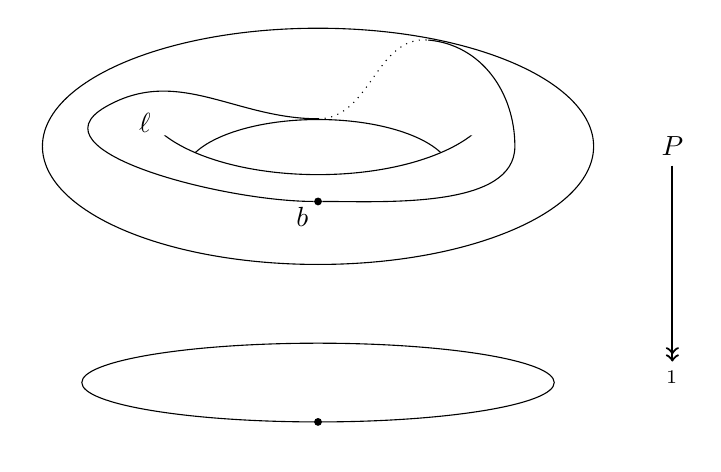
\begin{tikzpicture}
    \draw (0,0) ellipse (3 and .5);
    \draw (0,3) ellipse (3.5 and 1.5);
    \begin{scope}[yshift=4]
      \clip (-3,3) -- (-1.8,3) -- (-1.8,3.7) -- (1.8,3.7) -- (1.8,3) -- (3,3) -- (3,0) -- (-3,0) -- cycle;
      \draw[clip] (0,3.5) ellipse (2.25 and 1);
      \draw (0,2.5) ellipse (1.7 and .7);
    \end{scope}
    \node (P) at (4.5,3) {$P$};
    \node (S1) at (4.5,0) {$\Sn^1$};
    \draw[->>,thick] (P) -- (S1);
    \node[fill,circle,inner sep=1pt,label={below right:$\base$}] at (0,-.5) {};
    \node at (-2.6,.6) {$\lloop$};
    \node[fill,circle,\OPTblue,inner sep=1pt] (b) at (0,2.3) {};
    \node[\OPTblue] at (-.2,2.1) {$b$};
      \begin{scope}
        \draw[\OPTblue] (b) to[out=180,in=-150] (-2.7,3.5) to[out=30,in=180] (0,3.35);
        \draw[\OPTblue,dotted] (0,3.35) to[out=0,in=175] (1.4,4.35);
        \draw[\OPTblue] (1.4,4.35) to[out=-5,in=90] (2.5,3) to[out=-90,in=0,looseness=.8] (b);
      \end{scope}
      \node[\OPTblue] at (-2.2, 3.3) {$\ell$};
  \end{tikzpicture}
  \caption{$\Sn^1$ 的拓扑归纳原理}
  \label{fig:topS1ind}
\end{figure}

\begin{figure}
  \centering
  \begin{tikzpicture}
    \draw (0,0) ellipse (3 and .5);
    \draw (0,3) ellipse (3.5 and 1.5);
    \begin{scope}[yshift=4]
      \clip (-3,3) -- (-1.8,3) -- (-1.8,3.7) -- (1.8,3.7) -- (1.8,3) -- (3,3) -- (3,0) -- (-3,0) -- cycle;
      \draw[clip] (0,3.5) ellipse (2.25 and 1);
      \draw (0,2.5) ellipse (1.7 and .7);
    \end{scope}
    \node (P) at (4.5,3) {$P$};
    \node (S1) at (4.5,0) {$\Sn^1$};
    \draw[->>,thick] (P) -- (S1);
    \node[fill,circle,inner sep=1pt,label={below right:$\base$}] at (0,-.5) {};
    \node at (-2.6,.6) {$\lloop$};
    \node[fill,circle,\OPTblue,inner sep=1pt] (b) at (0,2.3) {};
      \node[\OPTblue] at (-.3,2.3) {$b$};
      \node[fill,circle,\OPTpurple,inner sep=1pt] (tb) at (0,1.8) {};
      % \draw[\OPTpurple,dashed] (b) to[out=0,in=0,looseness=5] (0,4) to[out=180,in=180] (tb);
      \draw[\OPTpurple,dashed] (b) arc (-90:90:2.9 and 0.85) arc (90:270:2.8 and 1.1);
      \begin{scope}
        \clip (b) -- ++(.1,0) -- (.1,1.8) -- ++(-.2,0) -- ++(0,-1) -- ++(3,2) -- ++(-3,0) -- (-.1,2.3) -- cycle;
        \draw[\OPTred,dotted,thick] (.2,2.07) ellipse (.2 and .57);
        \begin{scope}
          % \draw[clip] (b) -- ++(.1,0) |- (tb) -- ++(-.2,0) -- ++(0,-1) -| ++(3,3) -| (b);
          \clip (.2,0) rectangle (-2,3);
          \draw[\OPTred,thick] (.2,2.07) ellipse (.2 and .57);
        \end{scope}
      \end{scope}
      \node[\OPTred] at (1,1.2) {$\ell: \trans \lloop b=b$};
  \end{tikzpicture}
  \caption{$\Sn^1$ 的类型论归纳原理}
  \label{fig:ttS1ind}
\end{figure}

当然，我们期望能把 $P$ 取为常值类型族，从归纳原理推出递归原理。
这确实成立；不过，把 $\lloop$ 的非依值计算规则（涉及 $\apfunc f$）从依值计算规则（涉及 $\apdfunc f$）中导出，出乎意料地略有技巧。

\begin{lem}\label{thm:S1rec}
  \index{recursion principle!for S1@for $\Sn^1$}%
  \index{computation rule!for S1@for $\Sn^1$}%
  若给定类型 $A$，并给定 $a:A$ 与 $p:\id[A]aa$，则存在
  函数 $f:\Sn^1\to{}A$，满足
  \begin{align*}
    f(\base)&\defeq a \\
    \apfunc f(\lloop)&\defid p.
  \end{align*}
\end{lem}
\begin{proof}
  我们希望将 $\Sn^1$ 的归纳原理用于常值类型族 $(\lam{x} A): \Sn^1\to \UU$。
  为此需要的前提是：$(\lam{x} A)(\base) \jdeq A$ 中的一点（我们有，即 $a:A$），以及依值路径 $\dpath {x \mapsto A}{\lloop} a a$，等价地说是 $\transfib{x \mapsto A}{\lloop} a = a$。
  后者与类型 $\id[A]aa$（其中住留着 $p$）不同，但二者等价，因为由 \cref{thm:trans-trivial} 有 $\transconst{A}{\lloop}{a} : \transfib{x \mapsto A}{\lloop} a= a$。
  因此，给定 $a:A$ 与 $p:a=a$，可考虑复合
  \[\transconst{A}{\lloop}{a} \ct p:(\dpath {x \mapsto A}\lloop aa).\]
  应用归纳原理得到 $f:\Sn^1\to A$，并满足
  \begin{align}
    f(\base) &\jdeq a \qquad\text{and}\label{eq:S1recindbase}\\
    \apdfunc f(\lloop) &= \transconst{A}{\lloop}{a} \ct p.\label{eq:S1recindloop}
  \end{align}
  还需导出等式 $\apfunc f(\lloop)=p$。
  但由 \cref{thm:apd-const}，有
  \[\apdfunc f(\lloop) = \transconst{A}{\lloop}{f(\base)} \ct \apfunc f(\lloop).\]
  把它与~\eqref{eq:S1recindloop} 结合，并约去出现的 $\transconstf$（它们由~\eqref{eq:S1recindbase} 可知相同），即可得 $\apfunc f(\lloop)=p$。
\end{proof}

% Similarly, in this case we speak of defining $f$ by $f(\base)\defeq a$ and $\ap f \lloop \defid p$.
我们还有对应的唯一性原理。

\begin{lem}\label{thm:uniqueness-for-functions-on-S1}
  \index{uniqueness!principle, propositional!for functions on the circle}%
  设 $A$ 是一个类型，$f,g:\Sn^1\to{}A$ 是两个映射，并给定两条
  等式 $p,q$：
  \begin{align*}
    p:f(\base)&=_Ag(\base),\\
    q:\map{f}\lloop&=^{\lam{x} x=_Ax}_p\map{g}\lloop.
  \end{align*}
  则对所有 $x:\Sn^1$，都有 $f(x)=g(x)$。
\end{lem}
\begin{proof}
  我们把 $\Sn^1$ 的归纳原理应用于类型族 $P(x)\defeq(f(x)=g(x))$。
  当 $x$ 是 $\base$ 时，$p$ 正是所需数据。
  当 $x$ 沿 $\lloop$ 变化时，需要证明
  \(p=^{\lam{x} f(x)=g(x)}_{\lloop} p,\)
  而由 \cref{thm:transport-path,thm:dpath-path}，这可化约为 $q$。
\end{proof}

\index{universal!property!of S1@of $\Sn^1$}%
这两个引理推出圆的预期泛性质：

\begin{lem}\label{thm:S1ump}
  对任意类型 $A$，有自然等价
  \[ (\Sn^1 \to A) \;\eqvsym\;
  \sm{x:A} (x=x).
  \]
\end{lem}
\begin{proof}
  我们有一个规范函数 $f:(\Sn^1 \to A) \to \sm{x:A} (x=x)$，定义为 $f(g) \defeq (g(\base),\ap g \lloop)$。
  反方向上，有 $g:\sm{x:A} (x=x) \to (\Sn^1 \to A)$，它把一对 $(b,\ell)$ 送到由圆的递归原理给出的函数 $\Sn^1 \to A$。

  由递归原理的计算规则，$f \circ g \htpy \idfunc$。
  而 $g \circ f \htpy \idfunc$ 由唯一性原理得到，
  因为根据圆的递归原理计算规则，再次有 \((g \circ f)(\lloop) =^{\lam{x} x=_Ax}_{\refl{\base}} \lloop\)。
  因此，f 有一个拟逆，从而是等价。
\end{proof}

\index{type!circle|)}%

与 \cref{sec:htpy-inductive} 一样，我们可证明 \cref{thm:S1ump} 的结论等价于“存在一个带直谓计算规则的归纳原理”。
其他高阶归纳类型也满足与 \cref{thm:S1rec,thm:S1ump} 类似的引理；其证明我们一般留给读者。
下面继续看更多例子。
\section{区间}
\label{sec:interval}

\index{type!interval|(defstyle}%
\indexsee{interval!type}{type, interval}%
\define{区间}（记作 $\interval$）可能比圆更简单，是一个高阶归纳类型。
它由下列数据生成：
\begin{itemize}
\item 点 $\izero:\interval$，
\item 点 $\ione:\interval$，以及
\item 路径 $\seg : \id[\interval]\izero\ione$。
\end{itemize}
\index{recursion principle!for interval type}%
区间的递归原理断言：给定类型 $B$ 及
\begin{itemize}
\item 点 $b_0:B$，
\item 点 $b_1:B$，以及
\item 路径 $s:b_0=b_1$，
\end{itemize}
则存在函数 $f:\interval\to B$，满足 $f(\izero)\jdeq b_0$、$f(\ione)\jdeq b_1$，且 $\ap f \seg = s$。
\index{induction principle!for interval type}%
归纳原理断言：给定 $P:\interval\to\type$ 及
\begin{itemize}
\item 点 $b_0:P(\izero)$，
\item 点 $b_1:P(\ione)$，以及
\item 路径 $s:\dpath{P}{\seg}{b_0}{b_1}$，
\end{itemize}
则存在函数 $f:\prd{x:\interval} P(x)$，满足 $f(\izero)\jdeq b_0$、$f(\ione)\jdeq b_1$，且 $\apd f \seg = s$。

若只按同伦等价来看，区间本身并不太有趣：

\begin{lem}\label{thm:contr-interval}
  类型 $\interval$ 是可缩的。
\end{lem}

\begin{proof}
  我们证明对任意 $x:\interval$ 都有 $x=_\interval\ione$。也就是说，需要构造
  类型为 $\prd{x:\interval}(x=_\interval\ione)$ 的函数 $f$。先如下定义 $f$：
  \begin{alignat*}{2}
    f(\izero)&\defeq \seg  &:\izero&=_\interval\ione,\\
    f(\ione)&\defeq \refl\ione &:\ione &=_\interval\ione.
  \end{alignat*}
  还需定义 $\apd{f}\seg$，其类型必须是 $\seg =_\seg^{\lam{x} x=_\interval\ione}\refl \ione$。
  按定义该类型即 $\trans\seg\seg=_{\ione=_\interval\ione}\refl\ione$，又等价于 $\rev\seg\ct\seg=\refl\ione$。
  而该类型有一个规范元素：即“路径逆确为逆”的证明。
\end{proof}

不过，从类型论角度看，区间仍有一些有趣特征，这一点与经典同伦论中的拓扑区间类似。
例如，它使我们能较容易地证明函数外延性。
（当然，与 \cref{sec:univalence-implies-funext} 一样，在以下证明中我们暂时搁置全局的函数外延性公理假设。）

\begin{lem}\label{thm:interval-funext}
  \index{function extensionality!proof from interval type}%
  若 $f,g:A\to{}B$ 为两个函数，并且对每个 $x:A$ 都有 $f(x)=g(x)$，则
  在类型 $A\to{}B$ 中有 $f=g$。
\end{lem}

\begin{proof}
  设我们已有的证明为 $p:\prd{x:A}(f(x)=g(x))$。对每个 $x:A$ 定义
  函数 $\widetilde{p}_x:\interval\to{}B$ 如下：
  \begin{align*}
    \widetilde{p}_x(\izero) &\defeq f(x), \\
    \widetilde{p}_x(\ione) &\defeq g(x), \\
    \map{\widetilde{p}_x}\seg &\defid p(x).
  \end{align*}
  现在定义 $q:\interval\to(A\to{}B)$ 为
  \[q(i)\defeq(\lam{x} \widetilde{p}_x(i))\]
  那么 $q(\izero)$ 是函数 $\lam{x} \widetilde{p}_x(\izero)$；而 $\widetilde{p}_x(\izero)$ 按定义即 $f(x)$，故该函数等于 $f$。
  同理，$q(\ione)=g$，于是
  \[\map{q}\seg:f=_{(A\to{}B)}g \qedhere\]
\end{proof}

在 \cref{ex:funext-from-interval} 中，我们请读者由 \cref{thm:interval-funext} 完成完整函数外延性公理的证明。

\index{type!interval|)}%

\section{圆与球面}
\label{sec:circle}

\index{type!circle|(}%
我们已经讨论过：圆 $\Sn^1$ 是由下列构造子生成的高阶归纳类型
\begin{itemize}
\item 一个点 $\base:\Sn^1$，以及
\item 一条路径 $\lloop : {\id[\Sn^1]\base\base}$。
\end{itemize}
\index{induction principle!for S1@for $\Sn^1$}%
其归纳原理断言：给定 $P:\Sn^1\to\type$，以及 $b:P(\base)$ 与 $\ell :\dpath P \lloop b b$，则有 $f:\prd{x:\Sn^1} P(x)$，满足 $f(\base)\jdeq b$ 且 $\apd f \lloop = \ell$。
其非依值递归原理断言：给定 $B$ 及 $b:B$ 与 $\ell:b=b$，则有 $f:\Sn^1\to B$，满足 $f(\base)\jdeq b$ 且 $\ap f \lloop = \ell$。

我们注意到圆是非平凡的。

\begin{lem}\label{thm:loop-nontrivial}
  $\lloop\neq\refl{\base}$。
\end{lem}
\begin{proof}
  设 $\lloop=\refl{\base}$。
  由于对任意类型 $A$、任意 $x:A$ 与 $p:x=x$，都存在函数 $f:\Sn^1\to A$，由 $f(\base)\defeq x$ 与 $\ap f \lloop \defid p$ 定义，因此有
  \[p = f(\lloop) = f(\refl{\base}) = \refl{x}.\]
  这将推出每个类型都是集合，但我们已知这不成立（见 \cref{thm:type-is-not-a-set}）。
\end{proof}

圆还有下面这个有趣性质，可作为反例来源。

\begin{lem}\label{thm:S1-autohtpy}
  存在 $\prd{x:\Sn^1} (x=x)$ 的一个元素，它不等于 $x\mapsto \refl{x}$。
\end{lem}
\begin{proof}
  我们定义 $f:\prd{x:\Sn^1} (x=x)$，并使用 $\Sn^1$-归纳。
  当 $x$ 是 $\base$ 时，令 $f(\base)\defeq \lloop$。
  现在当 $x$ 沿 $\lloop$ 变化时（见 \cref{rmk:varies-along}），我们需要证明 $\transfib{x\mapsto x=x}{\lloop}{\lloop} = \lloop$。
  然而在 \cref{sec:compute-paths} 中我们观察到 $\transfib{x\mapsto x=x}{p}{q} = \opp{p} \ct q \ct p$，所以要证的是 $\opp{\lloop} \ct \lloop \ct \lloop = \lloop$。
  这通过约去逆元即可。

  为证明 $f\neq (x\mapsto \refl{x})$，只需证明 $f(\base) \neq \refl{\base}$。
  但 $f(\base)=\lloop$，故这正是上一引理。
\end{proof}

例如，这可将 \cref{thm:type-is-not-a-set} 推广：任何包含圆的宇宙都不可能是 1-类型。

\begin{cor}
  若类型 $\Sn^1$ 属于某个宇宙 \type，则 \type 不是 1-类型。
\end{cor}
\begin{proof}
  由泛等，\type 中的类型 $\Sn^1=\Sn^1$ 等价于 $\Sn^1$ 的自同构类型 $\eqv{\Sn^1}{\Sn^1}$，故只需证明 $\eqv{\Sn^1}{\Sn^1}$ 不是集合。
  \index{automorphism!of S1@of $\Sn^1$}%
  为此，只需证明其恒等类型 $\id[(\eqv{\Sn^1}{\Sn^1})]{\idfunc[\Sn^1]}{\idfunc[\Sn^1]}$ 不是纯命题。
  由于“是等价”本身是纯命题，该类型等价于 $\id[(\Sn^1\to\Sn^1)]{\idfunc[\Sn^1]}{\idfunc[\Sn^1]}$。
  再由函数外延性，它等价于 $\prd{x:\Sn^1} (x=x)$，而我们在 \cref{thm:S1-autohtpy} 已见该类型含有两个不相等元素。
\end{proof}

\index{type!circle|)}%

\index{type!2-sphere|(}%
\indexsee{sphere type}{type, sphere}%
我们还提到过：二维球面 $\Sn^2$ 应是由下列数据生成的高阶归纳类型
\symlabel{s2b}
\begin{itemize}
\item 一个点 $\base:\Sn^2$，以及
\item 一条二维路径 $\surf:\refl{\base} = \refl{\base}$，其位于 ${\base=\base}$ 中。
\end{itemize}
\index{recursion principle!for S2@for $\Sn^2$}%
$\Sn^2$ 的递归原理不难陈述：给定 $B$ 及 $b:B$ 与 $s:\refl b = \refl b$，则有 $f:\Sn^2\to B$，满足 $f(\base)\jdeq b$ 且 $\aptwo f \surf = s$。
这里“$\aptwo f \surf$”表示把 $f$ 的函子作用扩展到二维路径，其精确定义如下。

\begin{lem}\label{thm:ap2}
  给定 $f:A\to B$、$x,y:A$、$p,q:x=y$ 以及 $r:p=q$，可得路径 $\aptwo f r : \ap f p = \ap f q$。
\end{lem}
\begin{proof}
  由路径归纳，可设 $p\jdeq q$ 且 $r$ 为自反性。
  此时定义 $\aptwo f {\refl p} \defeq \refl{\ap f p}$ 即可。
\end{proof}

为了陈述一般归纳原理，我们需要该引理的依值函数版本，而这又需要“依值二维路径”的概念。
与之前一样，这种对象有多种定义方式；其中一种是通过二维版传送给出。

\begin{lem}\label{thm:transport2}
  给定 $P:A\to\type$、$x,y:A$、$p,q:x=y$ 以及 $r:p=q$，对任意 $u:P(x)$，有 $\transtwo r u : \trans p u = \trans q u$。
\end{lem}
\begin{proof}
  由路径归纳。
\end{proof}

现在设已给定 $x,y:A$、$p,q:x=y$、$r:p=q$，并且给定点 $u:P(x)$ 与 $v:P(y)$，以及依值路径 $h:\dpath P p u v$ 与 $k:\dpath P q u v$。
按我们对依值路径的定义，这即是 $h:\trans p u = v$ 与 $k:\trans q u = v$。
因此，把位于 $r$ 之上的依值 2-路径类型定义为
\[ (\dpath P r h k )\defeq (h = \transtwo r u \ct k). \]
是合理的。现在我们可陈述 \cref{thm:ap2} 的依值版本。

\begin{lem}\label{thm:apd2}
  给定 $P:A\to\type$、$x,y:A$、$p,q:x=y$、$r:p=q$，以及函数 $f:\prd{x:A} P(x)$，有
  $\apdtwo f r : \dpath P r {\apd f p}{\apd f q}$。
\end{lem}
\begin{proof}
  路径归纳。
\end{proof}

\index{induction principle!for S2@for $\Sn^2$}%
现在可陈述 $\Sn^2$ 的归纳原理：设给定 $P:\Sn^2\to\type$、$b:P(\base)$，以及 $s:\dpath Q \surf {\refl b}{\refl b}$，其中 $Q\defeq\lam{p} \dpath P p b b$。则存在函数 $f:\prd{x:\Sn^2} P(x)$，满足 $f(\base)\jdeq b$ 且 $\apdtwo f \surf = s$。

\index{type!2-sphere|)}%

当然，随着维度上升，这种显式写法会越来越复杂。
因此若要定义所有 $n$ 的 $n$-球面，我们需要更系统的思路。
一种办法是直接使用 $n$ 维环路\index{loop!n-@$n$-}，而非一般的 $n$ 维路径。\index{path!n-@$n$-}

\index{type!pointed}%
回忆 \cref{sec:equality} 中\emph{带点类型} $\type_*$ 以及 $n$ 重环路空间\index{loop space!iterated} $\Omega^n : \type_* \to \type_*$
（\cref{def:pointedtype,def:loopspace}）。现在可把
$n$-球面 $\Sn^n$ 定义为由下列数据生成的高阶归纳类型
\index{type!n-sphere@$n$-sphere}%
\begin{itemize}
\item 一个点 $\base:\Sn^n$，以及
\item 一个 $n$-环路 $\lloop_n : \Omega^n(\Sn^n,\base)$。
\end{itemize}
要为这种表示写出归纳原理，我们需要定义“依值 $n$-环路\indexdef{loop!dependent n-@dependent $n$-}”的概念，以及依值函数在 $n$-环路上的作用。
这部分留给读者（见 \cref{ex:nspheres}）；下一节我们将讨论另一种有时更易处理的球面定义方式。
\section{悬挂}
\label{sec:suspension}

\indexsee{type!suspension of}{suspension}%
\index{suspension|(defstyle}%
类型 $A$ 的\define{悬挂}是把 $A$ 的点变成路径（从而把 $A$ 中的路径变成 2-路径，依此类推）的泛方式。
它是一个类型 $\susp A$，由以下生成元给出:\footnote{这里与依值对类型的记号存在一个不太理想的冲突，后者当然也写作 $\Sigma$。
  不过通常可由上下文消歧。}
\begin{itemize}
\item 一个点 $\north:\susp A$，
\item 一个点 $\south:\susp A$，以及
\item 一个函数 $\merid:A \to (\id[\susp A]\north\south)$。
\end{itemize}
这些名称意在提示一种“球体”图像：有一个北极点、一个南极点，以及一族由 $A$ 参数化的子午线
\indexdef{pole}%
\indexdef{meridian}%
将两极连接起来。
确实，正如我们将看到的，若 $A=\Sn^1$，则其悬挂等价于通常球面 $\Sn^2$。

\index{recursion principle!for suspension}%
$\susp A$ 的递归原理表明：给定类型 $B$ 以及
\begin{itemize}
\item 点 $n,s:B$，和
\item 函数 $m:A \to (n=s)$，
\end{itemize}
则有函数 $f:\susp A \to B$，满足 $f(\north)\jdeq n$ 与 $f(\south)\jdeq s$，并且对任意 $a:A$ 有 $\ap f {\merid(a)} = m(a)$。
\index{induction principle!for suspension}%
同样地，归纳原理表明：给定 $P:\susp A \to \type$ 以及
\begin{itemize}
\item 点 $n:P(\north)$，
\item 点 $s:P(\south)$，以及
\item 对每个 $a:A$，路径 $m(a):\dpath P{\merid(a)}ns$，
\end{itemize}
则存在函数 $f:\prd{x:\susp A} P(x)$，满足 $f(\north)\jdeq n$、$f(\south)\jdeq s$，且对每个 $a:A$ 有 $\apd f {\merid(a)} = m(a)$。

关于悬挂的第一个观察是：它给出了圆的另一种定义方式。

\begin{lem}\label{thm:suspbool}
  \index{type!circle}%
  $\eqv{\susp\bool}{\Sn^1}$。
\end{lem}
\begin{proof}
  由递归定义 $f:\susp\bool\to\Sn^1$，使得 $f(\north)\defeq \base$ 且 $f(\south)\defeq\base$，同时规定 $\ap f{\merid(\bfalse)}\defid\lloop$ 而 $\ap f{\merid(\btrue)} \defid \refl{\base}$。
  由递归定义 $g:\Sn^1\to\susp\bool$，使得 $g(\base)\defeq \north$，并令 $\ap g \lloop \defid \merid(\bfalse) \ct \opp{\merid(\btrue)}$。
  现在证明 $f$ 与 $g$ 互为拟逆。

  先由归纳证明对任意 $x:\susp \bool$ 有 $g(f(x))=x$。
  若 $x\jdeq\north$，则 $g(f(\north)) \jdeq g(\base)\jdeq \north$，故取 $\refl{\north} : g(f(\north))=\north$。
  若 $x\jdeq\south$，则 $g(f(\south)) \jdeq g(\base)\jdeq \north$，我们取等式 $\merid(\btrue) : g(f(\south)) = \south$。
  还需说明：当 $x$ 沿 $\merid(y)$ 变化时（$y:\bool$），这些等式保持一致；也就是说，把 $\refl{\north}$ 沿 $\merid(y)$ 传送后得到 $\merid(\btrue)$。
  由路径空间中的传送与拉回纤维化可知，这等价于证明
  \[ \opp{\ap g {\ap f {\merid(y)}}} \ct \refl{\north} \ct \merid(y) = \merid(\btrue). \]
  当然可约去 $\refl{\north}$。
  再由 \bool-induction，可设 $y\jdeq \bfalse$ 或 $y\jdeq \btrue$。
  若 $y\jdeq \bfalse$，则有
  \begin{align*}
    \opp{\ap g {\ap f {\merid(\bfalse)}}} \ct \merid(\bfalse)
    &= \opp{\ap g {\lloop}} \ct \merid(\bfalse)\\
    &= \opp{(\merid(\bfalse) \ct \opp{\merid(\btrue)})} \ct \merid(\bfalse)\\
    &= \merid(\btrue) \ct \opp{\merid(\bfalse)} \ct \merid(\bfalse)\\
    &= \merid(\btrue)
  \end{align*}
  而若 $y\jdeq \btrue$，则有
  \begin{align*}
    \opp{\ap g {\ap f {\merid(\btrue)}}} \ct \merid(\btrue)
    &= \opp{\ap g {\refl{\base}}} \ct \merid(\btrue)\\
    &= \opp{\refl{\north}} \ct \merid(\btrue)\\
    &= \merid(\btrue).
  \end{align*}
  因而对所有 $x:\susp \bool$ 都有 $g(f(x))=x$。

  现在由归纳证明对任意 $x:\Sn^1$ 有 $f(g(x))=x$。
  若 $x\jdeq \base$，则 $f(g(\base))\jdeq f(\north)\jdeq\base$，故有 $\refl{\base} : f(g(\base))=\base$。
  还需说明：当 $x$ 沿 $\lloop$ 变化时，该等式保持不变，即沿 $\lloop$ 传送后仍是其自身。
  同样地，由路径空间中的传送与拉回纤维化，这等价于证明
  \[ \opp{\ap f {\ap g {\lloop}}} \ct \refl{\base} \ct \lloop = \refl{\base}.\]
  但我们有
  \begin{align*}
    \ap f {\ap g {\lloop}} &= \ap f {\merid(\bfalse) \ct \opp{\merid(\btrue)}}\\
    &= \ap f {\merid(\bfalse)} \ct \opp{\ap f {\merid(\btrue)}}\\
    &= \lloop \ct \refl{\base}
  \end{align*}
  故结论容易得到。
\end{proof}

从拓扑上看，两点空间 \bool 也称为\emph{0 维球面} $\Sn^0$。
（例如，它是 $\mathbb{R}^1$ 中到原点距离为 $1$ 的点所成空间，正如拓扑 1-球面是 $\mathbb{R}^2$ 中到原点距离为 $1$ 的点所成空间。）
因此，\cref{thm:suspbool} 可以形象地表述为 $\eqv{\susp\Sn^0}{\Sn^1}$。
\index{type!n-sphere@$n$-sphere|defstyle}%
\indexsee{n-sphere@$n$-sphere}{type, $n$-sphere}%
事实上，这一模式继续成立：我们可递归地定义全部球面
\begin{equation}\label{eq:Snsusp}
  \Sn^0 \defeq \bool
  \qquad\text{and}\qquad
  \Sn^{n+1} \defeq \susp \Sn^n.
\end{equation}
甚至还能再向下一维，定义 $\Sn^{-1}\defeq \emptyt$，并观察到 $\eqv{\susp\emptyt}{\bool}$。

若要严格证明这与上一节给出的 $\Sn^n$ 定义一致，需要把后一种定义写得更显式。
不过，我们可以证明这个递归定义具有与后一种定义所应具备的同样泛性质。
若 $(A,a_0)$ 与 $(B,b_0)$ 是有基点类型（基点常被省略），记 $\Map_*(A,B)$ 为保基点映射类型：
\index{based map}
\symlabel{based-maps}
\[ \Map_*(A,B) \defeq \sm{f:A\to B} (f(a_0)=b_0). \]
注意任意类型 $A$ 都可产生有基点类型 $A_+ \defeq A+\unit$，其基点为 $\inr(\ttt)$；这称为\emph{添上一个不交基点}。
\indexdef{basepoint!adjoining a disjoint}%
\index{disjoint!basepoint}%
\index{adjoining a disjoint basepoint}%

\begin{lem}
  对任意类型 $A$ 与有基点类型 $(B,b_0)$，有
  \[ \eqv{\Map_*(A_+,B)}{(A\to B)} \]
\end{lem}
注意右侧是从 $A$ 到 $B$ 的通常\emph{不保基点}函数类型。
\begin{proof}
  从左到右：给定 $f:A_+ \to B$ 与 $p:f(\inr(\ttt)) = b_0$，得到 $f\circ \inl : A \to B$。
  从右到左：给定 $g:A\to B$，定义 $g':A_+ \to B$，令 $g'(\inl(a))\defeq g(a)$ 且 $g'(\inr(u)) \defeq b_0$。
  这些操作互为拟逆，留给读者验证。
\end{proof}

特别地，注意 $\eqv{\bool}{\unit_+}$。
因此，对任意有基点类型 $B$，有
\[{\Map_*(\bool,B)} \eqvsym {(\unit \to B)}\eqvsym B.\]
%
现在回忆：环路空间\index{loop space}操作 $\Omega$ 作用在有基点类型上，定义为 $\Omega(A,a_0) \defeq (\id[A]{a_0}{a_0},\refl{a_0})$。
我们也可令悬挂 $\susp$ 作用在有基点类型上：$\susp(A,a_0)\defeq (\susp A,\north)$。

\begin{lem}\label{lem:susp-loop-adj}
  \index{universal!property!of suspension}%
  对有基点类型 $(A,a_0)$ 与 $(B,b_0)$，有
  \[ \eqv{\Map_*(\susp A, B)}{\Map_*(A,\Omega B)}.\]
\end{lem}
\addtocounter{thm}{1}           % Because we removed a numbered equation in commit 8f54d16
\begin{proof}
我们先观察如下等价链：
\begin{align*}
\Map_*(\susp A, B) & \defeq \sm{f:\susp A\to B} (f(\north)=b_0) \\
                   & \eqvsym \sm{f:\sm{b_n : B}{b_s : B} (A \to (b_n = b_s))} (\fst(f)=b_0) \\
                   & \eqvsym \sm{b_n : B}{b_s : B} \big(A \to (b_n = b_s)\big) \times (b_n=b_0) \\
                   & \eqvsym \sm{p : \sm{b_n : B} (b_n=b_0)}{b_s : B} (A \to (\fst(p) = b_s)) \\
                   & \eqvsym \sm{b_s : B} (A \to (b_0 = b_s))
\end{align*}
第一个等价来自悬挂的泛性质，即
\[ \Parens{\susp A \to B} \eqvsym \Parens{\sm{b_n : B} \sm{b_s : B} (A \to (b_n = b_s)) } \]
其中从右到左的函数由递归子给出（见 \cref{ex:susp-lump}）。
第二与第三个等价由 \cref{ex:sigma-assoc} 给出，并伴随分量重排。
最后一个等价由 \cref{thm:omit-contr} 得到，因为由 \cref{thm:contr-paths}，$\sm{b_n : B} (b_n=b_0)$ 是可缩的，其中心为 $(b_0, \refl{b_0})$。

接下来由下列等价链完成证明：
\begin{align*}
  \sm{b_s : B} (A \to (b_0 = b_s))
  &\eqvsym \sm{b_s : B}{g:A \to (b_0 = b_s)}{q:b_0 = b_s} (g(a_0) = q)\\
  &\eqvsym \sm{r : \sm{b_s : B}(b_0 = b_s)}{g:A \to (b_0 = \proj1(r))} (g(a_0) = \proj2(r))\\
  &\eqvsym \sm{g:A \to (b_0 = b_0)} (g(a_0) = \refl{b_0})\\
  &\jdeq \Map_*(A,\Omega B).
\end{align*}
与前面类似，第一和最后一个等价由 \cref{thm:omit-contr,thm:contr-paths} 给出，第二个由 \cref{ex:sigma-assoc} 与分量重排给出。
\end{proof}

\index{type!n-sphere@$n$-sphere|defstyle}%
特别地，对按~\eqref{eq:Snsusp} 定义的球面有
\index{universal!property!of Sn@of $\Sn^n$}%
\[ \Map_*(\Sn^n,B) \eqvsym \Map_*(\Sn^{n-1}, \Omega B) \eqvsym \cdots \eqvsym \Map_*(\bool,\Omega^n B) \eqvsym \Omega^n B. \]
因此，这些 $\Sn^n$ 具有我们所期望的泛性质，与 \cref{sec:circle} 中按 $n$ 重环路空间\index{loop space!iterated}直接定义的球面一致。

\index{suspension|)}%

\section{胞腔复形}
\label{sec:cell-complexes}

\index{cell complex|(defstyle}%
\index{CW complex|(defstyle}%
在经典拓扑中，\emph{胞腔复形}是通过沿边界不断粘附圆盘而得到的空间。
若要求 $n$ 维圆盘\index{disc}的边界只落在维数严格小于 $n$ 的圆盘中（即 $(n-1)$-骨架）\index{skeleton!of a CW-complex}，则称其为 \emph{CW 复形}。

任何有限 CW 复形都可表示成一个高阶归纳类型：把 $n$ 维圆盘转成 $n$ 维路径，并把附着\index{attaching map}映射的像拆分为源\index{source!of a path constructor}与目标\index{target!of a path constructor}，且两者都写成低维路径的复合。
我们在 \cref{sec:circle} 中对 $\Sn^1$ 与 $\Sn^2$ 的显式定义正是这种形式。

\index{torus}%
另一个例子是环面 $T^2$，其生成元为：
\begin{itemize}
\item 一个点 $b:T^2$，
\item 一条路径 $p:b=b$，
\item 另一条路径 $q:b=b$，以及
\item 一条 2-路径 $t: p\ct q = q \ct p$。
\end{itemize}
也许最直观的方式是从一个矩形出发：有四个顶点 $a,b,c,d$、四条边 $p,q,r,s$，其内部明显给出一条从 $p\ct q$ 到 $r\ct s$ 的 2-路径 $t$：
\begin{equation*}
  \xymatrix{
      a\ar@{=}[r]^p\ar@{=}[d]_r \ar@{}[dr]|{\Downarrow t} &
      b\ar@{=}[d]^q\\
      c\ar@{=}[r]_s &
      d
      }
\end{equation*}
然后把边 $r$ 与 $q$ 识别、边 $s$ 与 $p$ 识别，结果四个角也随之全部识别。
从拓扑上看，这一识别正好得到环面。

\index{induction principle!for torus}%
\index{torus!induction principle for}%
到目前为止我们写出的归纳原理里，环面的归纳原理最为棘手。
给定 $P:T^2\to\type$，要构造截面 $\prd{x:T^2} P(x)$，需要
\begin{itemize}
\item 一个点 $b':P(b)$，
\item 一条路径 $p' : \dpath P p {b'} {b'}$，
\item 一条路径 $q' : \dpath P q {b'} {b'}$，以及
\item 一条位于 $t$ 之上的 2-路径 $t'$，连接“复合”后的 $p'\ct q'$ 与 $q'\ct p'$。
\end{itemize}
要使最后一项有意义，我们需要先定义依值路径的复合运算，不过这并不困难。
随后归纳原理给出函数 $f:\prd{x:T^2} P(x)$，满足 $f(b)\jdeq b'$、$\apd f {p} = p'$、$\apd f {q} = q'$，以及类似“$\apdtwo f t = t'$”的条件。
然而按当前写法它并不良类型：首先，等式 $\apd f {p} = p'$ 与 $\apd f {q} = q'$ 不是判定等式；其次，$\apdfunc f$ 仅在同伦意义下保持路径连接。
细节留给读者（见 \cref{ex:torus}）。

当然，环面的另一种定义是 $T^2 \defeq \Sn^1 \times \Sn^1$（在 \cref{ex:torus-s1-times-s1} 中我们请读者验证两种定义等价）。
\index{Klein bottle}%
\index{projective plane}%
不过，胞腔复形式定义更容易推广到缺少此类描述的空间，例如 Klein bottle、projective plane 等。
但写出其归纳原理会越来越困难，需要定义依值 $n$-路径以及 $\apdfunc{}$ 在 $n$-路径上的作用。
幸运的是，一旦我们有了球面，就有办法绕开这一困难。

\section{轮毂与辐条}
\label{sec:hubs-spokes}

\indexsee{spoke}{hub and spoke}%
\index{hub and spoke|(defstyle}%

在拓扑中，人们通常说通过沿其 $(n-1)$ 维边界球粘附 $n$ 维圆盘来构造 CW 复形。
\index{attaching map}%
但还有另一种表述：粘入一个 $(n-1)$ 维球面的\emph{锥}\index{cone!of a sphere}。
也就是说，可把一个圆盘\index{disc}看作由一个锥点（“轮毂”）和一族子午线
\index{meridian}%
（“辐条”）组成，这些辐条连续地把该点连接到边界上的每个点，如 \cref{fig:hub-and-spokes} 所示。

\begin{figure}
  \centering
  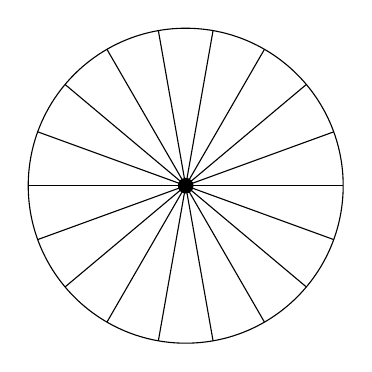
\begin{tikzpicture}
    \draw (0,0) circle (2cm);
    \foreach \x in {0,20,...,350}
      \draw[\OPTblue] (0,0) -- (\x:2cm);
    \node[\OPTblue,circle,fill,inner sep=2pt] (hub) at (0,0) {};
  \end{tikzpicture}
  \caption{由轮毂与辐条构成的 2-圆盘}
  \label{fig:hub-and-spokes}
\end{figure}

我们可以用这一思想，把含有 $n$ 维路径构造子（$n>1$）的高阶归纳类型，改写为只含 1 维路径构造子的类型。
要点在于：一个 $n$ 维路径可视为由某个 $(n-1)$ 维对象参数化的一族连续 1 维路径。
最简单的 $(n-1)$ 维参数对象是 $(n-1)$-球面，尽管在某些情形下别的对象可能更合适。
（回忆我们在 \cref{sec:suspension} 中已能用悬挂递归定义球面，而悬挂只涉及 1 维路径构造子。
事实上，悬挂也可看作这一思想的实例，因为它涉及一族由被悬挂类型参数化的 1 维路径。）

\index{torus}
例如，上一节的环面 $T^2$ 也可改定义为由以下生成元给出：
\begin{itemize}
\item 一个点 $b:T^2$，
\item 一条路径 $p:b=b$，
\item 另一条路径 $q:b=b$，
\item 一个点 $h:T^2$，以及
\item 对每个 $x:\Sn^1$，一条路径 $s(x) : f(x)=h$，其中 $f:\Sn^1\to T^2$ 定义为 $f(\base)\defeq b$ 且 $\ap f \lloop \defid p \ct q \ct \opp p \ct \opp q$。
\end{itemize}
这一版本环面的归纳原理表明：给定 $P:T^2\to\type$，要构造截面 $\prd{x:T^2} P(x)$，需要
\begin{itemize}
\item 一个点 $b':P(b)$，
\item 一条路径 $p' : \dpath P p {b'} {b'}$，
\item 一条路径 $q' : \dpath P q {b'} {b'}$，
\item 一个点 $h':P(h)$，以及
\item 对每个 $x:\Sn^1$，一条路径 $\dpath {P}{s(x)}{g(x)}{h'}$，其中 $g:\prd{x:\Sn^1} P(f(x))$ 定义为 $g(\base)\defeq b'$ 且 $\apd g \lloop \defid t(p' \ct q' \ct \opp{(p')} \ct \opp{(q')})$。
  在后式中，$\ct$ 表示依值路径连接，而 $t:\eqv{(\dpath{P}{\ap f \lloop}{b'}{b'})}{(\dpath{P\circ f}{\lloop}{b'}{b'})}$ 的定义留给读者。
\end{itemize}
注意这里不再需要依值 2-路径或 $\apdtwofunc{}$。
计算规则留给读者写出。

\begin{rmk}\label{rmk:spokes-no-hub}
或许会问：为什么要引入轮毂点 $h$？为何不直接连续地加入路径，把圆盘边界关联到边界\emph{上的}某一点，如 \cref{fig:spokes-no-hub} 所示？
但若不作额外修改，这样做并不可行。
因为给定某个 $f:\Sn^1 \to X$，若我们加入路径构造子把每个 $f(x)$ 连到 $f(\base)$，最终得到的更像 \cref{fig:spokes-no-hub-ii}：一个锥体的顶点被扭转后粘到其底面某点上。
问题在于，从 $f(\base)$ 到其自身所指定的路径未必是反身路径。
可以通过再加入一个 2 维路径构造子来修复，但使用独立轮毂可避免任何高于 $1$ 维的路径构造子。
\end{rmk}

\begin{figure}
  \centering
  \begin{minipage}{2in}
    \begin{center}
      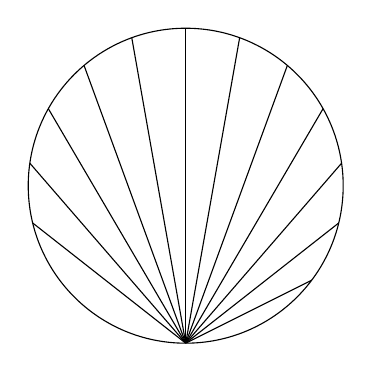
\begin{tikzpicture}
        \draw (0,0) circle (2cm);
        \clip (0,0) circle (2cm);
        \foreach \x in {0,15,...,165}
        \draw[\OPTblue] (0,-2cm) -- (\x:4cm);
      \end{tikzpicture}
    \end{center}
    \caption{无轮毂辐条}
    \label{fig:spokes-no-hub}
  \end{minipage}
  \qquad
  \begin{minipage}{2in}
    \begin{center}
      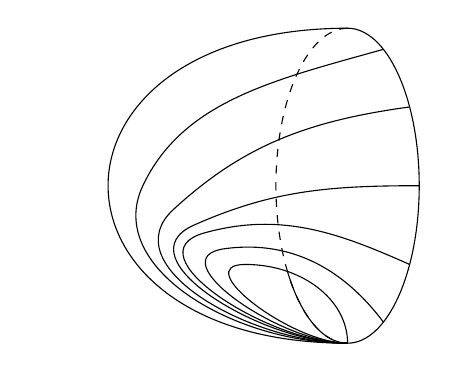
\begin{tikzpicture}[xscale=1.3]
        \draw (0,0) arc (-90:90:.7cm and 2cm) ;
        \draw[dashed] (0,4cm) arc (90:270:.7cm and 2cm) ;
        \draw[\OPTblue] (0,0) to[out=90,in=0] (-1,1) to[out=180,in=180] (0,0);
        \draw[\OPTblue] (0,4cm) to[out=180,in=180,looseness=2] (0,0);
        \path (0,0) arc (-90:-60:.7cm and 2cm) node (a) {};
        \draw[\OPTblue] (a.center) to[out=120,in=10] (-1.2,1.2) to[out=190,in=180] (0,0);
        \path (0,0) arc (-90:-30:.7cm and 2cm) node (b) {};
        \draw[\OPTblue] (b.center) to[out=150,in=20] (-1.4,1.4) to[out=200,in=180] (0,0);
        \path (0,0) arc (-90:0:.7cm and 2cm) node (c) {};
        \draw[\OPTblue] (c.center) to[out=180,in=30] (-1.5,1.5) to[out=210,in=180] (0,0);
        \path (0,0) arc (-90:30:.7cm and 2cm) node (d) {};
        \draw[\OPTblue] (d.center) to[out=190,in=50] (-1.7,1.7) to[out=230,in=180] (0,0);
        \path (0,0) arc (-90:60:.7cm and 2cm) node (e) {};
        \draw[\OPTblue] (e.center) to[out=200,in=70] (-2,2) to[out=250,in=180] (0,0);
        \clip (0,0) to[out=90,in=0] (-1,1) to[out=180,in=180] (0,0);
        \draw (0,4cm) arc (90:270:.7cm and 2cm) ;
      \end{tikzpicture}
    \end{center}
    \caption{无轮毂辐条 II}
    \label{fig:spokes-no-hub-ii}
  \end{minipage}
\end{figure}

\begin{rmk}
  \index{computation rule!propositional}%
  还需注意，这种把高维路径“翻译”为 1-路径的方法，不保留这些路径的判定计算规则，但保留其命题计算规则。
\end{rmk}

\index{cell complex|)}%
\index{CW complex|)}%

\index{hub and spoke|)}%

\section{推出}
\label{sec:colimits}

\index{type!limit}%
\index{type!colimit}%
\index{limit!of types}%
\index{colimit!of types}%
从范畴论角度看，任何基础系统的重要能力之一是构造极限与余极限。
在集合论基础中，这是集合的极限与余极限；而在我们这里，则是\emph{类型}的极限与余极限。
我们在 \cref{sec:universal-properties} 中见过：笛卡尔积类型具有类型范畴中积的正确泛性质；在 \cref{ex:coprod-ump} 中也见过：余积类型同样具有预期的泛性质。

如 \cref{sec:universal-properties} 所述，更一般的极限可用恒等类型与 $\Sigma$-类型构造，例如 $f:A\to C$ 与 $g:B\to C$ 的拉回\index{pullback}是 $\sm{a:A}{b:B} (f(a)=g(b))$（见 \cref{ex:pullback}）。
然而，更一般的\emph{余极限}要求识别来自不同类型的元素，而高阶归纳类型非常适合这一任务。
由于我们的全部构造都同伦不变，所有余极限必然都是\emph{同伦余极限}；为简洁起见，下文省略这一形容词。

本节讨论\emph{推出}，它也许是最简单且最有用的余极限之一。
确实，人们期望所有有限余极限（在某个合适的同伦意义下的“有限”）都可由推出与有限余积构造。
也可以直接用高阶归纳类型构造更一般的余极限，但这在技术上较繁琐，而且也并不完全令人满意，因为我们尚无一个良好的、完全一般的同伦相干图表概念。

\indexsee{type!pushout of}{pushout}%
\index{pushout|(defstyle}%
\index{span}%
设给定如下类型与函数构成的 span：
\[\Ddiag=\;\vcenter{\xymatrix{C \ar^g[r] \ar_f[d] & B \\ A & }}\]
该 span 的\define{推出}是高阶归纳类型 $A\sqcup^CB$，其呈示为
\begin{itemize}
\item 一个函数 $\inl:A\to A\sqcup^CB$，
\item 一个函数 $\inr:B \to A\sqcup^CB$，以及
\item 对每个 $c:C$，一条路径 $\glue(c):(\inl(f(c))=\inr(g(c)))$。
\end{itemize}
换言之，$A\sqcup^CB$ 是 $A$ 与 $B$ 的不交并，并且对每个 $c:C$ 额外给出一个见证，表明 $f(c)$ 与 $g(c)$ 相等。
递归原理表明：若 $D$ 是另一类型，我们可定义映射 $s:A\sqcup^CB\to{}D$，方法是给出
\begin{itemize}
\item 对每个 $a:A$，$s(\inl(a)):D$ 的值，
\item 对每个 $b:B$，$s(\inr(b)):D$ 的值，以及
\item 对每个 $c:C$，$\mapfunc{s}(\glue(c)):s(\inl(f(c)))=s(\inr(g(c)))$ 的值。
\end{itemize}
归纳原理留给读者表述。
它还蕴含如下唯一性原理：若 $s,s':A\sqcup^CB\to{}D$ 两个映射满足
\index{uniqueness!principle, propositional!for functions on a pushout}%
\begin{align*}
  s(\inl(a))&=s'(\inl(a))\\
  s(\inr(b))&=s'(\inr(b))\\
  \mapfunc{s}(\glue(c))&=\mapfunc{s'}(\glue(c))
  \qquad\text{(modulo the previous two equalities)}
\end{align*}
对每个 $a,b,c$ 均成立，则 $s=s'$。

为表述推出的泛性质，我们引入如下定义。

\begin{defn}\label{defn:cocone}
  给定跨图 $\Ddiag= (A \xleftarrow{f} C \xrightarrow{g} B)$ 与类型 $D$，一个\define{位于 $\Ddiag$ 下、顶点为 $D$ 的余锥}
  \indexdef{cocone}%
  \index{vertex of a cocone}%
  由函数 $i:A\to{}D$、$j:B\to{}D$ 以及同伦 $h : \prd{c:C} (i(f(c))=j(g(c)))$ 构成：
  \[\uppercurveobject{{ }}\lowercurveobject{{ }}\twocellhead{{ }}
  \xymatrix{C \ar^g[r] \ar_f[d] \drtwocell{^h} & B \ar^j[d] \\ A \ar_i[r] & D
  }\]
  我们记 $\cocone{\Ddiag}{D}$ 为所有此类余锥构成的类型，即
  \[ \cocone{\Ddiag}{D} \defeq
  \sm{i:A\to D}{j:B\to D} \prd{c:C} (i(f(c))=j(g(c))).
  \]
\end{defn}

当然，存在一个位于 $\Ddiag$ 下、顶点为 $A\sqcup^C B$ 的典范余锥，由 $\inl$、$\inr$ 与 $\glue$ 组成。
\[\uppercurveobject{{ }}\lowercurveobject{{ }}\twocellhead{{ }}
\xymatrix{C \ar^g[r] \ar_f[d] \drtwocell{^\glue\ \ } & B \ar^\inr[d] \\
  A \ar_-\inl[r] & A\sqcup^CB }\]
下面引理说明它是此类余锥中的泛者。

\begin{lem}\label{thm:pushout-ump}
  \index{universal!property!of pushout}%
  对任意类型 $E$，存在等价
  \[ (A\sqcup^C B \to E) \;\eqvsym\; \cocone{\Ddiag}{E}. \]
\end{lem}
\begin{proof}
  取任意类型 $E:\type$。
  有一个典范函数 $c_\sqcup$ 定义为
  \[\function{(A\sqcup^CB\to{}E)}{\cocone{\Ddiag}{E}}
  {t}{(t\circ{}\inl,t\circ{}\inr,\mapfunc{t}\circ{}\glue)}\]
  我们把它非正式写作 $t\mapsto\composecocone{t}c_\sqcup$。
  下证其为等价。

  首先，给定 $c=(i,j,h):\cocone{\mathscr{D}}{E}$，需构造映射
  $\mathsf{s}(c):A\sqcup^CB\to E$。
  \[\uppercurveobject{{ }}\lowercurveobject{{ }}\twocellhead{{ }}
  \xymatrix{C \ar^g[r] \ar_f[d] \drtwocell{^h} & B \ar^{j}[d] \\
    A \ar_-{i}[r] & E }\]
  映射 $\mathsf{s}(c)$ 定义如下
  \begin{align*}
    \mathsf{s}(c)(\inl(a))&\defeq i(a),\\
    \mathsf{s}(c)(\inr(b))&\defeq j(b),\\
    \mapfunc{\mathsf{s}(c)}(\glue(x))&\defid h(x).
  \end{align*}
  因而得到映射
\[\function{\cocone{\Ddiag}{E}}{(A\sqcup^CB\to{}E)}{c}{\mathsf{s}(c)}\]
并需证明它是 $t\mapsto{}\composecocone{t}c_\sqcup$ 的逆。
一方面，若 $c=(i,j,h):\cocone{\Ddiag}{E}$，则有
\begin{align*}
  \composecocone{\mathsf{s}(c)}c_\sqcup & =
  (\mathsf{s}(c)\circ\inl,\mathsf{s}(c)\circ\inr,
  \mapfunc{\mathsf{s}(c)}\circ\glue) \\
  & = (\lamu{a:A} \mathsf{s}(c)(\inl(a)),\;
  \lamu{b:B} \mathsf{s}(c)(\inr(b)),\;
  \lamu{x:C} \mapfunc{\mathsf{s}(c)}(\glue(x))) \\
  & = (\lamu{a:A} i(a),\;
  \lamu{b:B} j(b),\;
  \lamu{x:C} h(x)) \\
  & \jdeq (i, j, h) \\
  & = c.
\end{align*}
%
另一方面，若 $t:A\sqcup^CB\to{}E$，我们要证明
$\mathsf{s}(\composecocone{t}c_\sqcup)=t$。
对 $a:A$，有
\[\mathsf{s}(\composecocone{t}c_\sqcup)(\inl(a))=t(\inl(a))\]
因为 $\composecocone{t}c_\sqcup$ 的第一分量是 $t\circ\inl$。
同理，对 $b:B$ 有
\[\mathsf{s}(\composecocone{t}c_\sqcup)(\inr(b))=t(\inr(b))\]
且对 $x:C$ 有
\[\mapfunc{\mathsf{s}(\composecocone{t}c_\sqcup)}(\glue(x))
=\mapfunc{t}(\glue(x))\]
故 $\mathsf{s}(\composecocone{t}c_\sqcup)=t$。

这证明了 $c\mapsto\mathsf{s}(c)$ 是 $t\mapsto{}\composecocone{t}c_\sqcup$ 的拟逆，命题得证。
\end{proof}

若干标准同伦论构造都可表示为（同伦）推出。
\begin{itemize}
\item span $\unit \leftarrow A \to \unit$ 的推出是\define{悬挂} $\susp A$（见 \cref{sec:suspension}）。%
  \index{suspension}
\symlabel{join}
\item $A \xleftarrow{\proj1} A\times B \xrightarrow{\proj2} B$ 的推出称为 $A$ 与 $B$ 的\define{连接（join）}，记作 $A*B$。%
  \indexdef{join!of types}
\item $\unit \leftarrow A \xrightarrow{f} B$ 的推出称为 $f$ 的\define{锥}或\define{余纤维}。%
  \indexdef{cone!of a function}%
  \indexsee{mapping cone}{cone of a function}%
  \indexdef{cofiber of a function}%
\symlabel{wedge}
\item 若 $A$ 与 $B$ 分别带基点 $a_0:A$ 与 $b_0:B$，则 $A \xleftarrow{a_0} \unit \xrightarrow{b_0} B$ 的推出称为\define{楔和} $A\vee B$。%
  \indexdef{wedge}
\symlabel{smash}
\item 若 $A$ 与 $B$ 如上带基点，定义 $f:A\vee B \to A\times B$ 为 $f(\inl(a))\defeq (a,b_0)$ 与 $f(\inr(b))\defeq (a_0,b)$，并令 $\ap f \glue \defid \refl{(a_0,b_0)}$。
  则 $f$ 的锥称为\define{挤压积（smash 积）} $A\wedge B$。%
  \indexdef{smash product}
\end{itemize}
我们将在 \cref{cha:hlevels,cha:homotopy} 进一步讨论推出。

\begin{rmk}
  如 \cref{subsec:prop-trunc} 所述，记号 $\wedge$ 与 $\vee$（分别用于有基点空间的 smash 积与楔和）在逻辑中也常表示“与”和“或”。
  由于同伦类型论中的类型既可能像空间也可能像直谓，技术上确有潜在冲突；但它们很少同时扮演这两种角色，通常可由上下文消歧。
  此外，smash 积与楔和只作用于\emph{有基点}空间，而唯一的有基点纯命题是 $\top\jdeq\unit$；并且无论 $\wedge$、$\vee$ 取哪种含义，都有 $\unit\wedge \unit = \unit$ 与 $\unit\vee\unit=\unit$。
\end{rmk}

\index{pushout|)}%

\begin{rmk}
  注意余极限一般不保持截断性。
  例如，$\Sn^0$ 与 \unit 都是集合，但 $\unit \leftarrow \Sn^0 \to \unit$ 的推出是 $\Sn^1$，后者不是集合。
  因而若我们关心 $n$-类型范畴中的余极限（特别是集合范畴），就需要以某种方式对余极限做“截断”。
  我们将在 \cref{sec:hittruncations,cha:hlevels,cha:set-math} 回到这一点。
\end{rmk}

\section{截断}
\label{sec:hittruncations}

\index{truncation!propositional|(}%
在 \cref{subsec:prop-trunc} 中，我们把命题截断作为一种新的类型构造操作引入；
现在我们观察到，它可以作为高阶归纳类型的一个特例得到。
这将理解截断的问题化约为理解高阶归纳的问题，而后者至少可以进行系统化处理。
这也很有趣，因为它给出了第一个真正\emph{递归}的高阶归纳类型：其构造子从正在定义的类型中取输入（就像后继算子 $\suc:\nat\to\nat$ 那样）。

设 $A$ 是一个类型；我们将其命题截断 $\brck A$ 定义为由下列构造子生成的高阶归纳类型：
\begin{itemize}
\item 一个函数 $\bprojf : A \to \brck A$，以及
\item 对每个 $x,y:\brck A$，一条路径 $x=y$。
\end{itemize}
注意，第二个构造子按定义就是断言 $\brck A$ 是一个纯命题。
因此，$\brck A$ 的定义可解释为：$\brck A$ 由一个函数 $A\to\brck A$ 与“它是纯命题”这一事实自由生成。

这个高阶归纳定义的递归原理很容易写出：它说，给定任意类型 $B$ 及
\begin{itemize}
\item 一个函数 $g:A\to B$，以及
\item 对任意 $x,y:B$，一条路径 $x=_B y$，
\end{itemize}
就存在函数 $f:\brck A \to B$，满足
\begin{itemize}
\item 对所有 $a:A$，$f(\bproj a) \jdeq g(a)$，以及
\item 对任意 $x,y:\brck A$，函数 $\apfunc f$ 将 $\brck A$ 中给定的路径 $x=y$（在命题意义下）送到 $B$ 中给定的路径 $f(x) = f(y)$。
\end{itemize}
\index{recursion principle!for truncation}%
这恰好就是我们在 \cref{subsec:prop-trunc} 中陈述过的命题截断递归原理的假设：一个函数 $A\to B$ 且 $B$ 是纯命题；结论的第一部分也与那里完全一致。
第二部分（$\apfunc f$ 的作用）此前没有提到，但在这里它事实上是空的，因为 $B$ 是纯命题，因此其中\emph{任意}两条路径都会自动相等。

\index{induction principle!for truncation}%
$\brck A$ 也有归纳原理：给定任意 $B:\brck A \to \type$ 以及
\begin{itemize}
\item 一个函数 $g:\prd{a:A} B(\bproj a)$，以及
\item 对任意 $x,y:\brck A$ 与 $u:B(x)$、$v:B(y)$，一条依值路径 $q:\dpath{B}{p(x,y)}{u}{v}$，其中 $p(x,y)$ 是来自 $\brck A$ 第二个构造子的路径，
\end{itemize}
则存在 $f:\prd{x:\brck A} B(x)$，使得对 $a:A$ 有 $f(\bproj a)\jdeq g(a)$，并且还有另一条计算规则。
然而，由于任意两个纯命题之间（在同伦意义下）至多只有一个函数，这个归纳原理实际上并不太有用（另见 \cref{ex:prop-trunc-ind}）。

\index{truncation!propositional|)}%
\index{truncation!set|(}%

\index{set|(}%
不过，我们可以将这一想法推广，构造落在 $n$-类型中的类似截断，对任意 $n$ 都成立。
例如，我们可以定义\emph{$0$-截断} $\trunc0A$ 由下列构造子生成：
\begin{itemize}
\item 一个函数 $\tprojf0 : A \to \trunc0 A$，以及
\item 对每个 $x,y:\trunc0A$ 和每个 $p,q:x=y$，一条路径 $p=q$。
\end{itemize}
于是 $\trunc0A$ 由一个函数 $A\to \trunc0A$ 与“$\trunc0A$ 是集合”这一断言自由生成。
其自然归纳原理可表述为：给定 $B:\trunc0 A \to \type$ 及
\begin{itemize}
\item 一个函数 $g:\prd{a:A} B(\tproj0a)$，以及
\item 对任意 $x,y:\trunc0A$，若有 $z:B(x)$、$w:B(y)$，且对每个 $p,q:x=y$ 有 $r:\dpath{B}{p}{z}{w}$ 与 $s:\dpath{B}{q}{z}{w}$，再给出一个 $2$-路径 $v:\dpath{\dpath{B}{-}{z}{w}}{u(x,y,p,q)}{r}{s}$，其中 $u(x,y,p,q):p=q$ 由 $\trunc0A$ 的第二个构造子得到，
\end{itemize}
则存在 $f:\prd{x:\trunc0A} B(x)$，使得对所有 $a:A$，$f(\tproj0a)\jdeq g(a)$，并且 $\apdtwo{f}{u(x,y,p,q)}$ 就是上面指定的 $2$-路径。
（与命题情形一样，后一个条件最终也没有实质内容。）
不过由此我们可以证明一个更有用的归纳原理。

\begin{lem}\label{thm:trunc0-ind}
  设给定 $B:\trunc0 A \to \type$ 与 $g:\prd{a:A} B(\tproj0a)$，并假设每个 $B(x)$ 都是集合。
  则存在 $f:\prd{x:\trunc0A} B(x)$，使得对所有 $a:A$，$f(\tproj0a)\jdeq g(a)$。
\end{lem}
\begin{proof}
  只需为上文任意 $x,y,z,w,p,q,r,s$ 构造一个 $2$-路径 $v:\dpath{B}{u(x,y,p,q)}{r}{s}$。
  但依值 $2$-路径的定义表明，这就是纤维 $B(y)$ 中的一条普通 $2$-路径。
  由于 $B(y)$ 是集合，任意两条平行路径之间都存在 $2$-路径。
\end{proof}

这蕴含了所期望的泛性质。

\begin{lem}\label{thm:trunc0-lump}
  \index{universal!property!of truncation}%
  对任意集合 $B$ 与任意类型 $A$，与 $\tprojf0:A\to \trunc0A$ 复合给出一个等价
  \[ \eqvspaced{(\trunc0A\to B)}{(A\to B)}. \]
\end{lem}
\begin{proof}
  在 $B$ 为常值族时，\cref{thm:trunc0-ind} 的特例给出从右到左的映射，它是从左到右“与 $\tprojf0$ 复合”函数的右逆。
  为证明它也是左逆，取 $h:\trunc0A\to B$，并将 \cref{thm:trunc0-ind} 应用于复合 $a\mapsto h(\tproj0a)$，定义 $h':\trunc0A\to B$。
  于是 $h'(\tproj0a)=h(\tproj0a)$。

  但由于 $B$ 是集合，对任意 $x:\trunc0A$，类型 $h(x)=h'(x)$ 是纯命题，因此也是集合。
  因而由 \cref{thm:trunc0-ind}，由对任意 $a:A$ 有 $h'(\tproj0a)=h(\tproj0a)$ 可推出对任意 $x:\trunc0A$ 有 $h(x)=h'(x)$，从而 $h=h'$。
\end{proof}

\index{limit!of sets}%
\index{colimit!of sets}%
例如，这使我们能够构造集合的余极限。
我们已经见过：若 $A \xleftarrow{f} C \xrightarrow{g} B$ 是集合的一个跨图，那么推出 $A\sqcup^C B$ 可能不再是集合。
（例如若 $A$ 与 $B$ 都是 \unit，而 $C$ 是 \bool，则推出是 $\Sn^1$。）
不过通过截断，我们可以构造一个仍是集合、且对其他集合具有预期泛性质的推出。

\begin{lem}\label{thm:set-pushout}
  \index{universal!property!of pushout}%
  设 $A \xleftarrow{f} C \xrightarrow{g} B$ 是集合的一个跨图\index{span}。
  则对任意集合 $E$，有一个规范等价
  \[ \Parens{\trunc0{A\sqcup^C B} \to E} \;\eqvsym\; \cocone{\Ddiag}{E}. \]
\end{lem}
\begin{proof}
  复合 \cref{thm:pushout-ump,thm:trunc0-lump} 中的等价即可。
\end{proof}

我们将 $\trunc0{A\sqcup^C B}$ 称为 $f$ 与 $g$ 的\define{集合推出}
\indexdef{set-pushout}%
\index{pushout!of sets}
以区别于（同伦）推出 $A\sqcup^C B$。
另一种做法是修改 \cref{sec:colimits} 中推出的定义，把 $0$-截断构造子直接纳入其中，从而避免事后再截断。
对任意种类的集合余极限都可作类似说明；我们将在 \cref{cha:set-math} 中进一步讨论。

不过，尽管上述 $0$-截断定义可行（它给出我们想要的对象且与理论一致），仍有一些问题。
第一，它与高阶归纳类型的一般理论衔接得不够好。
一般来说，直接处理像我们给出的 $\trunc0A$ 第二个构造子这样的情形较为棘手，因为其\emph{输入}不仅涉及被定义类型的元素，还涉及其中的路径。

但这可以比较容易地绕开。
回忆在 \cref{sec:bool-nat} 中我们提到：若一个归纳类型 $W$ 的构造子需要“无限多个参数”（类型为 $W$），可改为接受一个类型为 $\nat\to W$ 的单参数。
这背后有一条一般原则：若构造子输入形式古怪，可使用一个辅助归纳类型（如 \nat）来参数化，从而把输入化为定义域为归纳类型的简单函数。

对于 $0$-截断，我们可以考虑辅助\emph{高阶}归纳类型 $S$，它由两个点 $a,b:S$ 和两条路径 $p,q:a=b$ 生成。
这样，$\trunc 0A$ 中那条可疑构造子可替换为下列无可指摘的构造子：
\begin{itemize}
\item 对每个 $f:S\to \trunc 0A$，给出一条路径 $\apfunc{f}(p) = \apfunc{f}(q)$。
\end{itemize}
因为给出从 $S$ 出发的映射，等价于给出两个点及其间两条平行路径，所以这会导出同样的归纳原理。

\index{set|)}%

\index{truncation!set|)}%
\index{truncation!n-truncation@$n$-truncation}%
然而，我们当前对 $0$-截断的定义还有一个更严重的问题：它不易推广。
若我们希望对所有 $n:\nat$ 统一描述“到 $n$-类型的 $n$-截断”定义方式，那么这种做法不可行，因为第二个构造子的参数个数会随 $n$ 增长。
因此在 \cref{sec:truncations} 中，我们将采用不同思路来构造这些截断，基于上面引入的类型 $S$ 与圆 $\Sn^1$ 等价这一观察。
该构造将 $0$-截断作为特例，并满足 \cref{thm:trunc0-ind,thm:trunc0-lump} 的广义版本。

\section{商}
\label{sec:set-quotients}

集合的一类特别重要的余极限是按关系取\emph{商}。
也就是说，设 $A$ 是集合，$R:A\times A \to \prop$ 是一族纯命题（一个\define{纯关系}）。
\indexdef{relation!mere}%
\indexdef{mere relation}%
它的商应当是如下两个投影的集合余等化子
\[ \tsm{a,b:A} R(a,b) \rightrightarrows A. \]
我们也可以直接描述它：定义高阶归纳类型 $A/R$，其生成子为
\index{set-quotient|(defstyle}%
\indexsee{quotient of sets}{set-quotient}%
\indexsee{type!quotient}{set-quotient}%
\begin{itemize}
\item 一个函数 $q:A\to A/R$；
\item 对每个满足 $R(a,b)$ 的 $a,b:A$，一个等式 $q(a)=q(b)$；以及
\item $0$-截断构造子：对所有 $x,y:A/R$ 和 $r,s:x=y$，有 $r=s$。
\end{itemize}
我们有时把这个高阶归纳类型 $A/R$ 称为 $A$ 关于 $R$ 的\define{集合商}，以强调它按定义产出一个集合。
（同伦理论中还有更一般的“商”概念，但大多超出本书范围。
不过在 \cref{sec:rezk} 中，我们会考虑类型按一个 $1$-群胚取“商”，这是比集合商高一层的情形。）

\begin{rmk}\label{rmk:quotient-of-non-set}
  实际上，在集合商的定义及其多数性质中，并不需要 $A$ 本身是集合。
  不过通常最有意义的仍是这个情形。
\end{rmk}

\begin{lem}\label{thm:quotient-surjective}
  函数 $q:A\to A/R$ 是满射。
\end{lem}
\begin{proof}
  我们要证明：对任意 $x:A/R$，仅仅存在某个 $a:A$ 使得 $q(a)=x$。
  使用 $A/R$ 的归纳原理即可。
  第一种情形是平凡的：若 $x$ 是 $q(a)$，那么当然仅仅存在一个 $a$ 使得 $q(a)=q(a)$。
  而且由于目标是纯命题，它自动尊重所有路径构造子，因此结论成立。
\end{proof}

现在我们可以证明集合商满足（集合）余等化子的预期泛性质。

\begin{lem}\label{thm:quotient-ump}
  对任意集合 $B$，与 $q$ 前复合给出一个等价
  \[ \eqvspaced{(A/R \to B)}{\Parens{\sm{f:A\to B} \prd{a,b:A} R(a,b) \to (f(a)=f(b))}}.\]
\end{lem}
\begin{proof}
  $(\blank\circ q)$ 的拟逆（从右到左）正是 $A/R$ 的递归原理。
  也就是说，给定 $f:A\to B$ 满足
  \narrowequation{\prd{a,b:A} R(a,b) \to (f(a)=f(b)),} 我们定义 $\bar f:A/R\to B$ 为 $\bar f(q(a))\defeq f(a)$。
  这个定义方程恰好说明 $(f\mapsto \bar f)$ 是 $(\blank\circ q)$ 的右逆。

  若它还要是左逆，就需证明：任意 $g:A/R\to B$ 与 $x:A/R$ 都满足 $g(x) = \overline{g\circ q}(x)$。
  但由 \cref{thm:quotient-surjective}，仅仅存在某个 $a$ 使得 $q(a)=x$。
  由于我们要证明的等式是纯命题，我们可假设纯然地存在这样的 $a$；于是
  $g(x) = g(q(a)) = \overline{g\circ q}(q(a)) = \overline{g\circ q}(x)$。
\end{proof}

当然，在经典情形中通常考虑 $R$ 是\define{等价关系}，即我们有
\indexdef{relation!equivalence}%
\indexsee{equivalence!relation}{relation, equivalence}%
%
\begin{itemize}
\item \define{反身性}：$\prd{a:A} R(a,a)$，
  \indexdef{reflexivity!of a relation}%
  \indexdef{relation!reflexive}%
\item \define{对称性}：$\prd{a,b:A} R(a,b) \to R(b,a)$，以及
  \indexdef{symmetry!of a relation}%
  \indexdef{relation!symmetric}%
\item \define{传递性}：$\prd{a,b,c:C} R(a,b) \times R(b,c) \to R(a,c)$。
  \indexdef{transitivity!of a relation}%
  \indexdef{relation!transitive}%
\end{itemize}
%
在这种情况下，集合商 $A/R$ 还有更多良好性质，我们将在 \cref{sec:piw-pretopos} 中看到：例如有 $R(a,b) \eqvsym (\id[A/R]{q(a)}{q(b)})$。
\symlabel{equivalencerelation}
我们常把等价关系 $R(a,b)$ 以中缀写作 $a\eqr b$。

按等价关系取商也可用其他方式构造。
集合论做法是把等价类看作 $A$ 的幂集\index{power set}的一个子集。
在类型论中我们也可模仿这种“impredicative”构造。
\index{impredicative!quotient}

\begin{defn}
  一个直谓 $P:A\to\prop$ 若满足仅仅存在某个 $a:A$，使得对所有 $b:A$ 都有 $\eqv{R(a,b)}{P(b)}$，
  则称 $P$ 是关系 $R : A \times A \to \prop$ 的一个\define{等价类}
  \indexdef{equivalence!class}%
  。
\end{defn}

由于 $R$ 与 $P$ 都是纯命题，等价 $\eqv{R(a,b)}{P(b)}$ 与蕴含 $R(a,b) \to P(b)$ 及 $P(b) \to R(a,b)$ 是同一回事。
当然，对任意 $a:A$，我们都有规范等价类 $P_a(b) \defeq R(a,b)$。

\begin{defn}\label{def:VVquotient}
  我们定义
  \begin{equation*}
    A\sslash R \defeq \setof{ P:A\to\prop | P \text{ is an equivalence class of } R}.
  \end{equation*}
  函数 $q':A\to A\sslash R$ 定义为 $q'(a) \defeq P_a$。
\end{defn}

\begin{thm}
  对 $A$ 上任意等价关系 $R$，类型 $A\sslash R$ 与集合商 $A/R$ 等价。
\end{thm}
\begin{proof}
  先注意，若 $R(a,b)$，则由于 $R$ 是等价关系，对任意 $c:A$ 都有 $R(a,c) \Leftrightarrow R(b,c)$。
  因而由泛等可得 $R(a,c) = R(b,c)$，再由函数外延性得 $P_a=P_b$，即 $q'(a)=q'(b)$。
  因此由 \cref{thm:quotient-ump}，我们得到诱导映射 $f:A/R \to A\sslash R$，满足 $f\circ q = q'$。

  我们证明 $f$ 既单又满，从而是等价。
  满性直接来自 $q'$ 的满性，而后者本质上由 $A\sslash R$ 的定义立即得到。
  对单射性，若 $f(x)=f(y)$，要证明纯命题 $x=y$，由 $q$ 的满性可设 $x=q(a)$、$y=q(b)$（某些 $a,b:A$）。
  则对任意 $c:A$，有 $R(a,c) = f(q(a))(c) = f(q(b))(c) = R(b,c)$，特别地 $R(a,b) = R(b,b)$。
  而 $R(b,b)$ 可居住（因 $R$ 为等价关系），故 $R(a,b)$ 也可居住。
  因此 $q(a)=q(b)$，于是 $x=y$。
\end{proof}

在 \cref{subsec:quotients} 中我们会给出该定理的另一种证明。
注意与 $A/R$ 不同，构造 $A\sslash R$ 会提升宇宙层级：若 $A:\UU_i$ 且 $R:A\to A\to \prop_{\UU_i}$，则在定义 $A\sslash R$ 时也必须使用 $\prop_{\UU_i}$ 以涵盖全部等价类，因此 $A\sslash R : \UU_{i+1}$。
当然，若在 \cref{subsec:prop-subsets} 中假设命题重定容公理，则可避免此问题。

\begin{rmk}\label{defn-Z}
前两种构造在一般性上提供了商，但在特定情形中可能有更简单构造。
例如，我们可把整数 \Z 定义为一个集合商
\indexdef{integers}%
\indexdef{number!integers}%
%
\[ \Z \defeq (\N \times \N)/{\eqr} \]
%
其中 $\eqr$ 是如下定义的等价关系
%
\[ (a,b) \eqr (c,d) \defeq (a + d = b + c). \]
%
换言之，序对 $(a,b)$ 表示整数 $a - b$。
但在这个例子里，等价类有\emph{规范代表}：即形如 $(n,0)$ 或 $(0,n)$ 的那些。
\end{rmk}

下面引理说明：当出现这种情形时，我们不需要前面两种一般商构造。
（函数 $r:A\to A$ 称为\define{幂等}
\indexdef{function!idempotent}%
\indexdef{idempotent!function}%
若 $r\circ r = r$。）

\begin{lem}\label{lem:quotient-when-canonical-representatives}
  设 $\eqr$ 是集合 $A$ 上的一个关系，并存在幂等函数 $r
  : A \to A$，使得对所有 $x, y: A$ 都有 $\eqv{(r(x) = r(y))}{(x \eqr y)}$。
  （这推出 $\eqr$ 是等价关系。）
  则类型
  %
  \begin{equation*}
    (A/{\eqr}) \defeq \Parens{\sm{x : A} r(x) = x}
  \end{equation*}
  %
  满足 $A$ 按 $\eqr$ 取集合商的泛性质，从而与其等价。
  换言之，存在映射 $q : A \to (A/{\eqr})$，使得对每个集合 $B$，与 $q$ 前复合诱导出等价
  %
  \begin{equation}
    \label{eq:quotient-when-canonical}
    \Parens{(A/{\eqr}) \to B} \eqvsym \Parens{\sm{g : A \to B} \prd{x, y : A} (x \eqr y) \to (g(x) = g(y))}.
  \end{equation}
\end{lem}

\begin{proof}
  设 $i : \prd{x : A} r(r(x)) = r(x)$ 见证 $r$ 的幂等性。
  映射 $q : A \to (A/{\eqr})$ 定义为 $q(x) \defeq (r(x), i(x))$。
  注意由于 $A$ 是集合，$q(x)=q(y)$ 当且仅当 $r(x)=r(y)$，故（由假设）当且仅当 $x \eqr y$。
  我们定义一个从左到右的映射 $e$（见 \eqref{eq:quotient-when-canonical}）为
  \[ e(f) \defeq (f \circ q, \nameless), \]
  %
  其中下划线 $\nameless$ 代表如下证明：若 $x, y : A$ 且 $x \eqr y$，则如上所见 $q(x)=q(y)$，从而 $f(q(x)) = f(q(y))$。
  为证明 $e$ 是等价，考虑反向映射 $e'$，定义为
  %
  \[ e'(g, s) (x,p) \defeq g(x). \]
  %
  任取 $f : (A/{\eqr}) \to B$，
  %
  \[ e'(e(f))(x, p) \jdeq f(q(x)) \jdeq f(r(x), i(x)) = f(x, p) \]
  %
  最后一个等式成立是因为 $p : r(x) = x$，故 $(x,p) = (r(x), i(x))$（由于 $A$ 是集合）。类似地可算得
  %
  \[ e(e'(g, s)) \jdeq e(g \circ \proj{1}) \jdeq (g \circ \proj{1} \circ q, {\nameless}). \]
  %
  因为 $B$ 是集合，我们不必关心 $\nameless$ 部分；而第一分量满足
  %
  \[ g(\proj{1}(q(x))) \jdeq g(r(x)) = g(x), \]
  %
  其中最后一个等式是因为 $r(x) \eqr x$，且由假设 $s$，$g$ 尊重 $\eqr$。
\end{proof}

\begin{cor}\label{thm:retraction-quotient}
  设 $p:A\to B$ 是集合之间的一个收缩。
  则 $B$ 是 $A$ 按下式定义的等价关系 $\eqr$ 的商：
  \[ (a_1 \eqr a_2) \defeq (p(a_1) = p(a_2)). \]
\end{cor}
\begin{proof}
  设 $s:B\to A$ 是 $p$ 的一个截面。
  则 $s\circ p : A\to A$ 是幂等映射，并满足该 $\eqr$ 下 \cref{lem:quotient-when-canonical-representatives} 的条件；而 $s$ 诱导出 $B$ 到其不动点集合的同构。
\end{proof}

\begin{rmk}\label{Z-quotient-by-canonical-representatives}
\cref{lem:quotient-when-canonical-representatives} 可应用于 \Z，其中幂等映射 $r : \N \times \N \to \N \times \N$
定义为
%
\begin{equation*}
  r(a, b) =
  \begin{cases}
    (a - b, 0) & \text{if $a \geq b$,} \\
    (0, b - a) & \text{otherwise.}
  \end{cases}
\end{equation*}
%
（即使在构造性语境下这也是良定义的，因为 \N 上关系 $\geq$ 是可判定的。）
因此，非负整数可规范表示为 $(k, 0)$，非正整数可规范表示为 $(0, m)$，其中 $k,m:\N$。
这种分情形给出下面关于整数的“归纳原理”，它将在 \cref{cha:homotopy} 中有用。
\index{natural numbers}%
（照例，我们把自然数 $n$ 与对应非负整数同一，即与 $(n,0):\N\times\N$ 在 \Z 中的像同一。）
\end{rmk}

\begin{lem}\label{thm:sign-induction}
  \index{integers!induction principle for}%
  \index{induction principle!for integers}%
  设 $P:\Z\to\type$ 是一个类型族，并且我们有
  \begin{itemize}
  \item $d_0: P(0)$,
  \item $d_+: \prd{n:\N} P(n) \to P(\suc(n))$，以及
  \item $d_- : \prd{n:\N} P(-n) \to P(-\suc(n))$.
  \end{itemize}
  则存在 $f:\prd{z:\Z} P(z)$，满足
  \begin{itemize}
    \item $f(0) = d_0$,
    \item 对所有 $n:\N$，$f(\suc(n)) = d_+(n,f(n))$，以及
    \item 对所有 $n:\N$，$f(-\suc(n)) = d_-(n,f(-n))$。
  \end{itemize}
\end{lem}
\begin{proof}
  在本证明中，令 $\Z$ 表示 $\sm{x:\N\times\N}(r(x)=x)$，其中 $r$ 为上述幂等映射。
  （然后我们可把结果传送到与之等价的任意 \Z 定义上。）
  令 $q:\N\times\N\to\Z$ 为商映射，按 \cref{lem:quotient-when-canonical-representatives} 定义为 $q(x) = (r(x),i(x))$。
  现在定义 $Q\defeq P\circ q:\N\times \N \to \type$。
  通过沿适当等式传送给定数据，我们得到
  \begin{align*}
    d'_0 &: Q(0,0)\\
    d'_+ &: \prd{n:\N} Q(n,0) \to Q(\suc(n),0)\\
    d'_- &: \prd{n:\N} Q(0,n) \to Q(0,\suc(n)).
  \end{align*}
  另外注意到由于 $q(n,m) = q(\suc(n),\suc(m))$，我们有诱导等价
  \[e_{n,m}:\eqv{Q(n,m)}{Q(\suc(n),\suc(m))}.\]
  接着可对 $x$ 作双重归纳，构造 $g:\prd{x:\N\times \N} Q(x)$：
  \begin{align*}
    g(0,0) &\defeq d'_0,\\
    g(\suc(n),0) &\defeq d'_+(n,g(n,0)),\\
    g(0,\suc(m)) &\defeq d'_-(m,g(0,m)),\\
    g(\suc(n),\suc(m)) &\defeq e_{n,m}(g(n,m)).
  \end{align*}
  现在有 $\proj1 : \Z \to \N\times\N$，且满足 $q\circ \proj1 = \idfunc$。
  特别地，有 $Q\circ \proj1 = P$，从而得到一族等价 $s:\prd{z:\Z} \eqv{Q(\proj1(z))}{P(z)}$。
  因此可定义 $f(z) = s(z,g(\proj1(z)))$，得到 $f:\prd{z:\Z} P(z)$，并可验证所需等式。
\end{proof}

我们有时把由 \cref{thm:sign-induction} 得到的函数 $f:\prd{z:\Z} P(z)$ 记为一种模式匹配语法，包含三个分支 $d_0$、$d_+$ 与 $d_-$：
\begin{align*}
  f(0) &\defid d_0\\
  f(\suc(n)) &\defid d_+(n,f(n))\\
  f(-\suc(n)) &\defid d_-(n,f(-n))
\end{align*}
这里使用 $\defid$ 而非 $\defeq$（就像我们处理高阶归纳类型路径构造子时那样），以表明 \cref{thm:sign-induction} 所蕴含的“计算”规则只是命题等式。
例如，用这种方式可对任意整数 $n$ 定义环路的 $n$ 次连接。

\begin{cor}\label{thm:looptothe}
  \indexdef{path!concatenation!n-fold@$n$-fold}%
  设 $A$ 是一个类型，$a:A$ 且 $p:a=a$。
  存在函数 $\prd{n:\Z} (a=a)$，记作 $n\mapsto p^n$，其定义为
  \begin{align*}
    p^0 &\defid \refl{a}\\
    p^{n+1} &\defid p^n \ct p
    & &\text{当 $n\ge 0$ 时}\\
    p^{n-1} &\defid p^n \ct \opp p
    & &\text{当 $n\le 0$ 时。}
  \end{align*}
\end{cor}

我们将在 \cref{sec:free-algebras,sec:field-rati-numb} 中进一步讨论整数。

\index{set-quotient|)}%
\section{代数}
\label{sec:free-algebras}

除了构造球面与胞腔复形这类高维对象之外，高阶归纳类型在只研究集合时同样非常有用。
我们在 \cref{thm:set-pushout} 中已经见过一个例子：它们使我们能够构造任意集合图式的余极限，而这在 \cref{cha:typetheory} 的基础类型论中是做不到的。
当我们研究带代数结构的集合时，高阶归纳类型也非常有用。

本节我们以\emph{群}为贯穿示例：这对多数数学家都很熟悉，且体现了本质现象（后续章节也会用到）。
不过，我们所说的大部分内容同样适用于任何代数结构。

\index{monoid|(}%

\begin{defn}
  \define{幺半群}
  \indexdef{monoid}%
  是一个集合 $G$，并配有
  \begin{itemize}
  \item 一个\emph{乘法}
    \indexdef{multiplication!in a monoid}%
    \indexdef{multiplication!in a group}%
    函数 $G\times G\to G$，中缀记作 $(x,y) \mapsto x\cdot y$；以及
  \item 一个\emph{单位元}
    \indexdef{unit!of a monoid}%
    \indexdef{unit!of a group}%
    元素 $e:G$；并满足
  \item 对任意 $x:G$，有 $x\cdot e = x$ 与 $e\cdot x = x$；以及
  \item 对任意 $x,y,z:G$，有 $x\cdot (y\cdot z) = (x\cdot y)\cdot z$。
    \index{associativity!in a monoid}%
    \index{associativity!in a group}%
  \end{itemize}
  \define{群}
  \indexdef{group}%
  是一个幺半群 $G$，并配有
  \begin{itemize}
  \item 一个\emph{求逆}
    函数 $i:G\to G$，记作 $x\mapsto \opp x$；且满足
    \index{inverse!in a group}%
  \item 对任意 $x:G$，有 $x\cdot \opp x = e$ 与 $\opp x \cdot x = e$。
  \end{itemize}
\end{defn}

\begin{rmk}\label{rmk:infty-group}
注意我们要求群是集合。
我们也可考虑更一般的“$\infty$-群”%
\index{.infinity-group@$\infty$-group}
概念，它不必是集合，但这会把讨论带离当前主题。
按我们现在的定义，预期得到的“群论”会与集合论数学中的群论相似（但须注意：除非假设 \LEM{}，它将是“构造性”群论）。\index{mathematics!constructive}
\end{rmk}

\begin{eg}
  自然数 \N 在加法下是一个幺半群，单位元为 $0$；在乘法下也是一个幺半群，单位元为 $1$。
  若以显然方式定义整数 \Z 上的算术运算，则如常见情形，它在加法下是群、在乘法下是幺半群（当然还是一个环）。
  例如，若 $u, v \in \Z$ 分别由 $(a,b)$ 与 $(c,d)$ 表示，则 $u + v$ 由 $(a + c, b + d)$ 表示，$-u$ 由 $(b, a)$ 表示，而 $u v$ 由 $(a c + b d, a d + b c)$ 表示。
\end{eg}

\begin{eg}\label{thm:homotopy-groups}
  我们在 \cref{sec:equality} 中实际上已观察到：若 $(A,a)$ 是带点类型，则其环路空间\index{loop space} $\Omega(A,a)\defeq (\id[A]aa)$ 具有群的全部结构，只是一般并非集合。
  它应当是 \cref{rmk:infty-group} 所说意义下的“$\infty$-群”，但我们也可通过截断把它变成一个群。
  具体地，我们定义 $A$ 在基点 $a:A$ 处的\define{基本群}
  \indexsee{group!fundamental}{fundamental group}%
  \indexdef{fundamental!group}%
  为
  \[\pi_1(A,a)\defeq \trunc0{\Omega(A,a)}.\]
  它继承群结构；例如，乘法 $\pi_1(A,a) \times \pi_1(A,a) \to \pi_1(A,a)$ 可由路径连接经双重截断归纳定义。

  更一般地，$(A,a)$ 的\define{$n^{\mathrm{th}}$ 同伦群}
  \index{homotopy!group}%
  \indexsee{group!homotopy}{homotopy group}%
  定义为 $\pi_n(A,a)\defeq \trunc0{\Omega^n(A,a)}$。
  \index{loop space!iterated}%
  当 $n\ge 1$ 时，$\pi_n(A,a) = \pi_1(\Omega^{n-1}(A,a))$，所以它也是群。
  （当 $n=0$ 时，$\pi_0(A) \jdeq \trunc0 A$，它不是群。）
  另外，Eckmann--Hilton 论证 \index{Eckmann--Hilton argument}（\cref{thm:EckmannHilton}）蕴含：若 $n\ge 2$，则 $\pi_n(A,a)$ 是\emph{阿贝尔}\index{group!abelian}群，即对所有 $x,y$ 都有 $x\cdot y = y\cdot x$。
  \cref{cha:homotopy} 在很大程度上就是研究这些群。
\end{eg}

\index{algebra!free}%
\index{free!algebraic structure}%
群论中的一个重要概念是由一个集合生成的\emph{自由群}，更一般地，是由生成元\index{generator!of a group}和关系\emph{给出表示}的群。
在类型论中人们早已知道：\emph{某些}自由代数对象可以用\emph{普通}归纳类型定义。
\symlabel{lst-freemonoid}%
\indexdef{type!of lists}%
\indexsee{list type}{type, of lists}%
\index{monoid!free|(}%
例如，集合 $A$ 上的自由幺半群可与元素为 $A$ 的\emph{有限列表} \index{finite!lists, type of} 类型 $\lst A$ 同一，它由下列构造子归纳生成：
\begin{itemize}
\item 一个构造子 $\nil:\lst A$，以及
\item 对每个 $\ell:\lst A$ 与 $a:A$，一个元素 $\cons(a,\ell):\lst A$。
\end{itemize}
我们有显然的嵌入 $\eta : A\to \lst A$，定义为 $a\mapsto \cons(a,\nil)$。
$\lst A$ 上的幺半群运算是列表连接，按递归定义为
\begin{align*}
  \nil \cdot \ell &\defeq \ell\\
  \cons (a,\ell_1) \cdot \ell_2 &\defeq \cons(a, \ell_1\cdot\ell_2).
\end{align*}
利用 $\lst A$ 的归纳原理，直接可证 $\lst A$ 是集合，且列表连接满足结合律
\index{associativity!of list concatenation}%
并以 $\nil$ 为单位元。
因此，$\lst A$ 是幺半群。

\begin{lem}\label{thm:free-monoid}
  \indexsee{free!monoid}{monoid, free}%
  对任意集合 $A$，类型 $\lst A$ 是 $A$ 上的自由幺半群。
  换言之，对任意幺半群 $G$，与 $\eta$ 复合给出一个等价
  \[ \eqv{\hom_{\mathrm{Monoid}}(\lst A,G)}{(A\to G)}, \]
  其中 $\hom_{\mathrm{Monoid}}(\blank,\blank)$ 表示幺半群同态（保持乘法和单位元的函数）构成的集合。
  \indexdef{homomorphism!monoid}%
  \indexdef{monoid!homomorphism}%
\end{lem}
\begin{proof}
  给定 $f:A\to G$，我们递归定义 $\bar{f}:\lst A \to G$：
  \begin{align*}
    \bar{f}(\nil) &\defeq e\\
    \bar{f}(\cons(a,\ell)) &\defeq f(a) \cdot \bar{f}(\ell).
  \end{align*}
  通过归纳可直接证明 $\bar{f}$ 是幺半群同态，且 $f\mapsto \bar f$ 是 $(\blank\circ \eta)$ 的拟逆；见 \cref{ex:free-monoid}。
\end{proof}

\index{monoid!free|)}%

这种自由幺半群的构造可行，本质上是因为自由幺半群元素具有可计算的规范形（即有限列表）。
但其他自由（以及表示）代数结构，例如群，一般并不具有\emph{可计算}的规范形。
例如，群表示中字词相等的判定在算法上\index{algorithm}是不可判定的。
不过我们仍可把自由代数对象描述为\emph{高阶}归纳类型：只需把所有公理等式作为路径构造子直接断言。

\indexsee{free!group}{group, free}%
\index{group!free|(}%
例如，设 $A$ 是集合，定义高阶归纳类型 $\freegroup{A}$，其生成子如下。
\begin{itemize}
\item 一个函数 $\eta:A\to \freegroup{A}$。
\item 一个函数 $m: \freegroup{A} \times \freegroup{A} \to \freegroup{A}$。
\item 一个元素 $e:\freegroup{A}$。
\item 一个函数 $i:\freegroup{A} \to \freegroup{A}$。
\item 对每个 $x,y,z:\freegroup{A}$，一个等式 $m(x,m(y,z)) = m(m(x,y),z)$。
\item 对每个 $x:\freegroup{A}$，等式 $m(x,e) = x$ 与 $m(e,x) = x$。
\item 对每个 $x:\freegroup{A}$，等式 $m(x,i(x)) = e$ 与 $m(i(x),x) = e$。
\item $0$-截断构造子：对任意 $x,y:\freegroup{A}$ 与 $p,q:x=y$，有 $p=q$。
\end{itemize}
第一个构造子说明 $A$ 映入 $\freegroup{A}$。
接下来的三个赋予 $\freegroup{A}$ 群运算：乘法、单位元和求逆。
再后面的三个构造子断言群公理：结合律\index{associativity}、单位律和逆元律。
最后一个构造子断言 $\freegroup{A}$ 是集合。

因此，$\freegroup{A}$ 是一个群。
并且可以直接证明：

\begin{thm}
  \index{universal!property!of free group}%
  $\freegroup{A}$ 是 $A$ 上的自由群。
  换言之，对任意（集合意义下的）群 $G$，与 $\eta:A\to \freegroup{A}$ 复合确定一个等价
  \[ \hom_{\mathrm{Group}}(\freegroup{A},G) \eqvsym (A\to G) \]
  其中 $\hom_{\mathrm{Group}}(\blank,\blank)$ 表示两个群之间的群同态构成的集合。
  \indexdef{group!homomorphism}%
  \indexdef{homomorphism!group}%
\end{thm}
\begin{proof}
  高阶归纳类型 $\freegroup{A}$ 的递归原理\emph{恰好}说明：若 $G$ 是群且给定 $f:A\to G$，则有 $\bar{f}:\freegroup{A} \to G$。
  其计算规则说明 $\bar{f}\circ \eta \jdeq f$，且 $\bar f$ 是群同态。
  因而 $(\blank\circ \eta) :  \hom_{\mathrm{Group}}(\freegroup{A},G) \to (A\to G)$ 有一个右逆。
  再利用 $\freegroup{A}$ 的归纳原理，可直接证明它也是左逆。
\end{proof}

\index{acceptance}
值得退一步看看我们刚做了什么。
我们在\emph{没有}给出自由群显式构造的情况下，证明了任意集合上的自由群存在。
本质上我们所做的几乎只是写下它应满足的泛性质。
在集合论里，我们可借助伴随函子定理\index{adjoint!functor theorem}之类“黑箱”得到类似结论；而类型论把这类构造直接内置到数学基础中。

当然，给出自由代数结构的具体描述有时也有用。
对自由群而言，我们可借助商给出一个。
考虑 $\lst{A+A}$，其中在 $A+A$ 中把 $\inl(a)$ 记作 $a$，把 $\inr(a)$ 记作 $\hat{a}$（意在表示 $a$ 的形式逆元）。
$\lst{A+A}$ 的元素就是 $A$ 上自由群的\emph{字}。

\begin{thm}
  设 $A$ 是集合，令 $\freegroupx{A}$ 为 $\lst{A+A}$ 按下列关系取集合商所得。
  \begin{align*}
    (\dots,a_1,a_2,\widehat{a_2},a_3,\dots) &=
    (\dots,a_1,a_3,\dots)\\
    (\dots,a_1,\widehat{a_2},a_2,a_3,\dots) &=
    (\dots,a_1,a_3,\dots).
  \end{align*}
  则 $\freegroupx{A}$ 也是集合 $A$ 上的自由群。
\end{thm}
\begin{proof}
  先证明 $\freegroupx{A}$ 是群。
  我们已知 $\lst{A+A}$ 是幺半群；我们断言该幺半群结构可下降到商上。
  通过双重商递归定义 $\freegroupx{A} \times \freegroupx{A} \to \freegroupx{A}$；只需检查由给定关系生成的等价关系被列表连接保持。
  同理，结合律与单位律可由商归纳证明。

  为在 $\freegroupx{A}$ 中定义逆元，先在列表上递归定义 $\mathsf{reverse}:\lst B\to\lst B$：
  \begin{align*}
    \mathsf{reverse}(\nil) &\defeq \nil,\\
    \mathsf{reverse}(\cons(b,\ell))&\defeq \mathsf{reverse}(\ell)\cdot \cons(b,\nil).
  \end{align*}
  现在通过商递归定义 $i:\freegroupx{A}\to \freegroupx{A}$：对列表 $\ell:\lst{A+A}$，先交换两份 $A$，再反转列表。
  该操作保持关系，因此可下降到商上。
  接着可归纳证明对 $x:\freegroupx{A}$ 有 $i(x) \cdot x = e$。
  首先由商归纳可设 $x$ 来自某个 $\ell:\lst{A+A}$，再作列表归纳；若记 $q:\lst{A+A}\to \freegroupx{A}$ 为商映射，则各情形为
  \begin{align*}
    i(q(\nil)) \ct q(\nil) &= q(\nil) \ct q(\nil)\\
    &= q(\nil)\\
    i(q(\cons(a,\ell))) \ct q(\cons(a,\ell)) &= i(q(\ell)) \ct q(\cons(\hat{a},\nil)) \ct q(\cons(a,\ell))\\
    &= i(q(\ell)) \ct q(\cons(\hat{a},\cons(a,\ell)))\\
    &= i(q(\ell)) \ct q(\ell)\\
    &= q(\nil). \tag{由归纳假设}
  \end{align*}
  （这里略去了一些关于列表连接行为等相当明显的引理。）

  至此完成了 $\freegroupx{A}$ 为群的证明。
  现在若 $G$ 是任意群并给定函数 $f:A\to G$，可定义 $A+A\to G$：在第一份 $A$ 上取 $f$，在第二份 $A$ 上取 $f$ 与 $G$ 的求逆映射复合。
  由 $G$ 为幺半群，可得幺半群同态 $\lst{A+A} \to G$。
  又因 $G$ 是群，此映射尊重上述关系，故可下降为映射 $\freegroupx{A}\to G$。
  直接可证它是群同态，且是限制到 $A$ 上等于 $f$ 的唯一群同态。
\end{proof}

\index{monoid|)}%

若 $A$ 具有可判定相等性\index{decidable!equality}（例如假设排中律），则定义 $\freegroupx{A}$ 的商可由 \cref{lem:quotient-when-canonical-representatives} 那样的幂等映射得到。
我们称一个字（即 $\lst{A+A}$ 的元素）是\define{约化的}
\indexdef{reduced word in a free group}
若它不含相邻的 $(a,\hat a)$ 或 $(\hat a,a)$ 配对。

当 $A$ 具有可判定相等性时，定义字的\define{约化}
\index{reduction!of a word in a free group}%
是直接的；它是生成相应商的幂等映射。细节留给读者。

若 $A\defeq \unit$（其相等性可判定），则约化字只能全由 $\ttt$ 组成，或全由 $\hat{\ttt}$ 组成。
因此，$\unit$ 上的自由群与整数 \Z 等价：$0$ 对应 $\nil$，正整数 $n$ 对应由 $n$ 个 $\ttt$ 组成的约化字，负整数 $(-n)$ 对应由 $n$ 个 $\hat{\ttt}$ 组成的约化字。
当然，也可以直接证明 \Z 满足 $\freegroup{\unit}$ 的泛性质。

\begin{rmk}\label{thm:freegroup-nonset}
  在构造 $\freegroup{A}$ 与 $\freegroupx{A}$ 及证明其泛性质时，我们从未用到 $A$ 是集合这一假设。
  因此实际上可以对任意类型构造自由群。
  比较泛性质可得 $\eqv{\freegroup{A}}{\freegroup{\trunc0A}}$。
\end{rmk}

\index{group!free|)}%

\index{algebra!colimits of}%
我们也可用高阶归纳类型构造代数对象的余极限。
例如，设 $f:G\to H$ 与 $g:G\to K$ 是群同态。
它们在群范畴中的推出称为\define{并合自由积}
\indexdef{amalgamated free product}%
\indexdef{free!product!amalgamated}%
$H *_G K$，可构造为由下列数据生成的高阶归纳类型：
\begin{itemize}
\item 函数 $h:H\to H *_G K$ 与 $k:K\to H *_G K$。
\item 如 $\freegroup{A}$ 定义中那样的群运算与群公理。
\item 断言 $h$ 与 $k$ 是群同态的公理。
\item 对 $x:G$，有 $h(f(x)) = k(g(x))$。
\item $0$-截断构造子。
\end{itemize}
另一方面，它也可显式构造为 $\lst{H+K}$ 按如下关系取集合商：
\begin{align*}
  (\dots, x_1, x_2, \dots) &= (\dots, x_1\cdot x_2, \dots)
  & &\text{for $x_1,x_2:H$}\\
  (\dots, y_1, y_2, \dots) &= (\dots, y_1\cdot y_2, \dots)
  & &\text{for $y_1,y_2:K$}\\
  (\dots, 1_G, \dots) &= (\dots, \dots) &&  \\
  (\dots, 1_H, \dots) &= (\dots, \dots) &&  \\
  (\dots, f(x), \dots) &= (\dots, g(x), \dots)
  & &\text{for $x:G$.}
\end{align*}
证明留给读者。
在特殊情形 $G$ 是平凡群时，最后一条关系可省略，得到\define{自由积}
\indexdef{free!product}%
$H*K$，即群范畴中的余积。
（该记号不幸与类型\emph{连接}的记号冲突，如 \cref{sec:colimits}，但语境一般可消歧。）

\index{presentation!of a group}%
注意由\emph{表示}定义的群可视为余极限的特例。
设给定集合（更一般可为类型）$A$，以及一对函数 $R\rightrightarrows \freegroup{A}$。
我们把 $R$ 看作“关系”类型，这两个函数给每条关系指定其所要等同的两个字。
例如在表示 $\langle a \mid a^2 = e \rangle$ 中，可取 $A\defeq \unit$ 且 $R\defeq \unit$，两条态射 $R\rightrightarrows \freegroup{A}$ 分别选出列表 $(a,a)$ 与空列表 $\nil$。
由自由群的泛性质，得到一对群同态 $\freegroup{R} \rightrightarrows \freegroup{A}$。
它们在群范畴中的余等化子（构造方式与推出相同）就是该\emph{表示}所定义的群。

\mentalpause

注意，这些构造只适用于\emph{代数}理论，\index{theory!algebraic} 即其公理是关于给定符号\index{signature!of an algebraic theory}中的变量、常元、运算所写的（全称量化）方程。
它们也可修改后适用于所谓\emph{本质代数理论}：\index{theory!essentially algebraic} 其运算在由先前运算间等式指定的定义域上部分定义。
例如它们不适用于域论：其中“取逆”运算在由先前运算间\emph{远离关系} $\#$ 所指定的定义域 $\setof{x | x \mathrel{\#} 0}$ 上部分定义，见 \cref{RD-inverse-apart-0}。
确实，众所周知域范畴没有始对象。
\index{initial!field}%

另一方面，这些构造同样适用于\emph{无穷元}\index{infinitary!algebraic theory}代数理论，即其“运算”可接受无限多个输入。
在这种情形下，若不假设选择公理，自由代数或代数余极限未必能表示为简单商。
这意味着高阶归纳类型显著增强了构造性类型论（未必体现在证明论强度上，而体现在实践能力上）；在某些方面它们甚至强于 Zermelo--Fraenkel\index{set theory!Zermelo--Fraenkel} 集合论（不含选择）~\cite{blass:freealg}。
% We will see an example of this in \cref{sec:ordinals}.
\section{展平引理}
\label{sec:flattening}

正如我们将在 \cref{cha:homotopy} 中看到的，当把高阶归纳类型与泛等结合起来时，会出现非常惊人的现象。
其主要机制是：若 $W$ 是高阶归纳类型且 \UU 是类型宇宙，那么可利用 $W$ 的递归原理定义一个类型族 $P:W\to \UU$。
当处理递归原理中对应 $W$ 的路径构造子的分支时，我们需要在 \UU 中提供路径，而这正是泛等发挥作用之处。

例如，设有一个类型 $X$ 与一个自等价 $e:\eqv X X$。
那么可用 $\Sn^1$-递归定义类型族 $P:\Sn^1 \to \UU$：
\begin{equation*}
  P(\base) \defeq X
  \qquad\text{且}\qquad
  \ap P\lloop \defid \ua(e).
\end{equation*}
于是 $X$ 作为纤维 $P(\base)$ 出现在 $P$ 的基点之上。
自等价 $e$ 在 $P$ 中隐藏得更深一些，但下面引理说明可通过沿 \lloop 传送把它提取出来。

\begin{lem}\label{thm:transport-is-given}
  给定 $B:A\to\type$ 与 $x,y:A$，并有路径 $p:x=y$ 及等价 $e:\eqv{B(x)}{B(y)}$，满足 $\ap{B}p = \ua(e)$，则对任意 $u:B(x)$ 都有
  \begin{align*}
    \transfib{B}{p}{u} &= e(u).
  \end{align*}
\end{lem}
\begin{proof}
  应用 \cref{thm:transport-is-ap}，有
  \begin{align*}
    \transfib{B}{p}{u} &= \idtoeqv(\ap{B}p)(u)\\
    &= \idtoeqv(\ua(e))(u)\\
    &= e(u).\qedhere
  \end{align*}
\end{proof}

我们此前已经见过用递归定义类型族：在 \cref{sec:compute-coprod,sec:compute-nat} 中，我们用它来刻画（普通）归纳类型的恒等类型。
在 \cref{cha:homotopy} 中，我们将用类似思想计算高阶归纳类型的同伦群。

本节给出关于这类类型族的一条一般性引理，后文会用到。
我们称其为\define{展平引理}：
\indexdef{flattening lemma}%
\indexdef{lemma!flattening}%
它说，如果 $P:W\to\UU$ 如上递归定义，则其总空间 $\sm{x:W} P(x)$ 与一个“展平后的”高阶归纳类型等价；该类型的构造子可由 $W$ 的构造子与 $P$ 的定义推导得到。
（从范畴论观点看，$\sm{x:W} P(x)$ 是 $P$ 的“Grothendieck\index{Grothendieck construction} 构造”，而展平引理把其泛性质表达为一个“lax\index{lax colimit} 余极限”。由于同伦类型论中的类型（如 $W$）在范畴上对应 $\infty$-群胚（因为所有路径可逆），在这里 lax 余极限与 pseudo 余极限是一致的。）

我们在此证明展平引理的一个一般情形，它直接推出许多特例，也指示了证明其他情形的方法。
设 $A,B:\type$ 与 $f,g:B\to{}A$，并令高阶归纳类型 $W$ 由下列构造子生成：
\begin{itemize}
\item $\cc:A\to{}W$，以及
\item $\pp:\prd{b:B} (\cc(f(b))=_W\cc(g(b)))$。
\end{itemize}
于是 $W$ 是 $f$ 与 $g$ 的\define{（同伦）余等化子}
\indexdef{coequalizer}%
\indexdef{type!coequalizer}%
。
利用二元和（余积）与依值和（$\Sigma$-类型），许多有趣的非递归高阶归纳类型都可表示成这种形式。
所有点构造子都打包进类型 $A$，所有路径构造子都打包进类型 $B$。
例如：
\begin{itemize}
\item 圆 $\Sn^1$ 可由 $A\defeq \unit$、$B\defeq \unit$ 表示，且 $f,g$ 都取恒等。
\item $j:X\to Y$ 与 $k:X\to Z$ 的推出可由 $A\defeq Y+Z$、$B\defeq X$ 表示，其中 $f\defeq \inl \circ j$、$g\defeq \inr\circ k$。
\end{itemize}
现在再假设
\begin{itemize}
\item $C:A\to\type$ 是 $A$ 上的类型族，且
\item $D:\prd{b:B}\eqv{C(f(b))}{C(g(b))}$ 是 $B$ 上的一族等价。
\end{itemize}
递归地定义类型族 $P : W\to\type$：
\begin{align*}
  P(\cc(a)) &\defeq C(a)\\
  \map{P}{\pp(b)} &\defid \ua(D(b)).
\end{align*}
令 \Wtil 为由下列构造子生成的高阶归纳类型：
\begin{itemize}
\item $\cct:\prd{a:A} C(a) \to \Wtil$，以及
\item $\ppt:\prd{b:B}{y:C(f(b))} (\cct(f(b),y)=_{\Wtil}\cct(g(b),D(b)(y)))$。
\end{itemize}

展平引理如下：

\begin{lem}[展平引理]\label{thm:flattening}
  在上述情形中，有
  \[ \eqvspaced{\Parens{\sm{x:W} P(x)}}{\widetilde{W}}. \]
\end{lem}

\index{universal!property!of dependent pair type}%
如上所述，这个等价可视为表达 $\sm{x:W} P(x)$ 作为 $P$ 在 $W$ 上的一个“lax\index{lax colimit} 余极限”的泛性质。
它也可视为余极限\emph{稳定性与下降}性质的一部分，而这刻画了高阶拓扑斯。%
\index{.infinity1-topos@$(\infty,1)$-topos}%
\index{stability!and descent}%

\cref{thm:flattening} 的证明占据本节余下部分。
它有些技术性，初读时可以跳过。
但它也是“证据相关数学”的一个好例子，
\index{mathematics!proof-relevant}%
因此我们建议在二读时仔细看。

思路是证明 $\sm{x:W} P(x)$ 与 \Wtil 具有同样的泛性质。
我们先证明它带有与构造子 $\cct$、$\ppt$ 对应的数据。

\begin{lem}\label{thm:flattening-cp}
  存在函数
  \begin{itemize}
  \item $\cct':\prd{a:A} C(a) \to \sm{x:W} P(x)$，以及
  \item $\ppt':\prd{b:B}{y:C(f(b))} \Big(\cct'(f(b),y)=_{\sm{w:W}P(w)}\cct'(g(b),D(b)(y))\Big)$。
  \end{itemize}
\end{lem}
\begin{proof}
  第一个很简单；定义 $\cct'(a,x) \defeq (\cc(a),x)$，并注意由定义有 $P(\cc(a))\jdeq C(a)$。
  对第二个，设给定 $b:B$ 与 $y:C(f(b))$；我们需要给出等式
  \[ (\cc(f(b)),y) = (\cc(g(b)),D(b)(y)). \]
  由于已有 $\pp(b):\cc(f(b))=\cc(g(b))$，按 $\Sigma$-类型中的等式，只需给出等式 $\trans{\pp(b)}{y} = D(b)(y)$。
  而这由 \cref{thm:transport-is-given} 与 $P$ 的定义立得。
\end{proof}

下面的引理说明：要定义一个 $\sm{w:W} P(w)$ 上类型族的截面，只需给出与 \Wtil 情形相同形状的数据。

\begin{lem}\label{thm:flattening-rect}
  设 $Q:\big(\sm{x:W} P(x)\big) \to \type$ 是类型族，并且给定
  \begin{itemize}
  \item $c : \prd{a:A}{x:C(a)} Q(\cct'(a,x))$，以及
  \item $p : \prd{b:B}{y:C(f(b))} \Big(\trans{\ppt'(b,y)}{c(f(b),y)} = c(g(b),D(b)(y))\Big)$. %_{Q(\cct'(g(b),D(b)(y)))}
  \end{itemize}
  则存在 $k:\prd{z:\sm{w:W} P(w)} Q(z)$，使得 $k(\cct'(a,x)) \jdeq c(a,x)$。
\end{lem}
\begin{proof}
  设给定 $w:W$ 与 $x:P(w)$；我们需构造元素 $k(w,x):Q(w,x)$。
  对 $w$ 作归纳，只需考虑两种情形。
  当 $w\jdeq \cc(a)$ 时，$x:C(a)$，因此有所需的 $c(a,x):Q(\cc(a),x)$。
  （定义的这一部分也保证了所述计算规则成立。）

  现在需证明：对任意 $b:B$，该定义在沿 $\pp(b)$ 传送下保持。
  由于我们为所有 $w:W$ 定义的是函数类型 $\prd{x:P(w)} Q(w,x)$，由 \cref{thm:dpath-forall}，只需证明对任意 $y:C(f(b))$ 有
  \[ \transfib{Q}{\pairpath(\pp(b),\refl{\trans{\pp(b)}{y}})}{c(f(b),y)} = c(g(b),\trans{\pp(b)}{y}). \]
  令 $q:\trans{\pp(b)}{y} = D(b)(y)$ 为由 \cref{thm:transport-is-given} 得到的路径。
  则有
  \begin{align}
    c(g(b),\trans{\pp(b)}{y})
    &= \transfib{x\mapsto Q(\cct'(g(b),x))}{\opp{q}}{c(g(b),D(b)(y))}
    \tag{by $\opp{\apdfunc{x\mapsto c(g(b),x)}(\opp q)}$} \\
    &= \transfib{Q}{\apfunc{x\mapsto \cct'(g(b),x)}(\opp q)}{c(g(b),D(b)(y))}
    \tag{by \cref{thm:transport-compose}}.
  \end{align}
  因此只需证明
  \begin{multline*}
    \Transfib{Q}{\pairpath(\pp(b),\refl{\trans{\pp(b)}{y}})}{c(f(b),y)} = {}\\
    \Transfib{Q}{\apfunc{x\mapsto \cct'(g(b),x)}(\opp q)}{c(g(b),D(b)(y))}.
  \end{multline*}
  将右侧传送移到另一边并合并两次传送，这等价于
  %
  \begin{narrowmultline*}
    \Transfib{Q}{\pairpath(\pp(b),\refl{\trans{\pp(b)}{y}}) \ct
      \apfunc{x\mapsto \cct'(g(b),x)}(q)}{c(f(b),y)} =
    \narrowbreak
    c(g(b),D(b)(y)).
  \end{narrowmultline*}
  %
  但我们有
  \begin{multline*}
    \pairpath(\pp(b),\refl{\trans{\pp(b)}{y}}) \ct \apfunc{x\mapsto \cct'(g(b),x)}(q)
    = {} \\
    \pairpath(\pp(b),\refl{\trans{\pp(b)}{y}}) \ct \pairpath(\refl{\cc(g(b))},q)
    = \pairpath(\pp(b),q)
    = \ppt'(b,y)
  \end{multline*}
  所以由假设 $p(b,y)$（其类型为
  \[ \transfib{Q}{\ppt'(b,y)}{c(f(b),y)} = c(g(b),D(b)(y)). \qedhere \]
  ）即可完成构造。
\end{proof}

\cref{thm:flattening-rect} \emph{几乎}给出了 $\sm{w:W}P(w)$ 与 \Wtil 相同的归纳原理。
缺失的是等式 $\apdfunc{k}(\ppt'(b,y)) = p(b,y)$。
要证明它，需要分析 \cref{thm:flattening-rect} 的证明，而那当然就是 $k$ 的定义本身。

这应当可行，但事实证明我们只需要非依值递归原理的计算规则。
因此下面给出一个稍简单的直接递归子构造，以及其计算规则的证明。

\begin{lem}\label{thm:flattening-rectnd}
  设 $Q$ 是一个类型，并且给定
  \begin{itemize}
  \item $c : \prd{a:A} C(a) \to Q$，以及
  \item $p : \prd{b:B}{y:C(f(b))} \Big(c(f(b),y) =_Q c(g(b),D(b)(y))\Big)$。
  \end{itemize}
  则存在 $k:\big(\sm{w:W} P(w)\big) \to Q$，使得 $k(\cct'(a,x)) \jdeq c(a,x)$。
\end{lem}
\begin{proof}
  与 \cref{thm:flattening-rect} 一样，我们通过对 $w:W$ 归纳来定义 $k(w,x)$。
  当 $w\jdeq \cc(a)$ 时，定义 $k(\cc(a),x)\defeq c(a,x)$。
  现在由 \cref{thm:dpath-arrow}，只需考虑在 $b:B$ 与 $y:C(f(b))$ 下的复合路径
  \begin{equation}\label{eq:flattening-rectnd}
    \transfib{x\mapsto Q}{\pp(b)}{c(f(b),y)}
    = c(g(b),\transfib{P}{\pp(b)}{y})
  \end{equation}
  %
  它定义为下列复合
  %
  \begin{align}
    \transfib{x\mapsto Q}{\pp(b)}{c(f(b),y)}
    &= c(f(b),y) \tag{by \cref{thm:trans-trivial}}\\
    &= c(g(b),D(b)(y)) \tag{by $p(b,y)$}\\
    &= c(g(b),\transfib{P}{\pp(b)}{y}). \tag{by \cref{thm:transport-is-given}}
  \end{align}
  计算规则 $k(\cct'(a,x)) \jdeq c(a,x)$ 与先前一样由定义给出。
\end{proof}

为得到第二条计算规则，我们需要下面引理。

\begin{lem}\label{thm:ap-sigma-rect-path-pair}
  设 $Y:X\to\type$ 是类型族，$k:(\sm{x:X}Y(x)) \to Z$ 逐分量定义为 $k(x,y) \defeq d(x)(y)$，其中 $d:\prd{x:X} Y(x)\to Z$ 是柯里化函数。
  对任意 $s:\id[X]{x_1}{x_2}$、任意 $y_1:Y(x_1)$、$y_2:Y(x_2)$ 及路径 $r:\trans{s}{y_1}=y_2$，路径
  \[\apfunc k (\pairpath(s,r)) :k(x_1,y_1) = k(x_2,y_2)\]
  等于下列复合路径：
  \begin{align}
    k(x_1,y_1)
    &\jdeq d(x_1)(y_1) \notag\\
    &= \transfib{x\mapsto Z}{s}{d(x_1)(y_1)}
    \tag{by $\opp{\text{(\cref{thm:trans-trivial})}}$}\\
    &= \transfib{x\mapsto Z}{s}{d(x_1)(\trans{\opp s}{\trans{s}{y_1}})}
    \notag\\
    &= \big(\transfib{x\mapsto (Y(x)\to Z)}{s}{d(x_1)}\big)(\trans{s}{y_1})
    \tag{by~\eqref{eq:transport-arrow}}\\
    &= d(x_2)(\trans{s}{y_1})
    \tag{by $\happly(\apdfunc{d}(s))(\trans{s}{y_1}$}\\
    &= d(x_2)(y_2)
    \tag{by $\apfunc{d(x_2)}(r)$}\\
    &\jdeq k(x_2,y_2).
    \notag
  \end{align}
\end{lem}
\begin{proof}
  对 $s$ 与 $r$ 作路径归纳后，两边都化为自反路径。
\end{proof}

乍看之下，\cref{thm:ap-sigma-rect-path-pair} 的陈述似乎很复杂，而证明却很简单，这看起来有些意外。
复杂性的原因在于要保证陈述是良类型的：$\apfunc k (\pairpath(s,r))$ 与声称与之相等的复合路径必须有相同的起点和终点。
一旦做到这一点，证明就可由路径归纳直接完成。

\begin{lem}\label{thm:flattening-rectnd-beta-ppt}
  在 \cref{thm:flattening-rectnd} 的情形下，有 $\apfunc{k}(\ppt'(b,y)) = p(b,y)$。
\end{lem}
\begin{proof}
  回忆 $\ppt'(b,y) \defeq \pairpath(\pp(b),q)$，其中 $q:\trans{\pp(b)}{y} = D(b)(y)$ 来自 \cref{thm:transport-is-given}。
  因此，由于 $k$ 是逐分量定义的，我们可用 \cref{thm:ap-sigma-rect-path-pair} 计算 $\apfunc{k}(\ppt'(b,y))$，取
  \begin{align*}
    x_1 &\defeq \cc(f(b)) & y_1 &\defeq y\\
    x_2 &\defeq \cc(g(b)) & y_2 &\defeq D(b)(y)\\
    s &\defeq \pp(b)      &   r &\defeq q.
  \end{align*}
  柯里化函数 $d:\prd{w:W} P(w) \to Q$ 是通过对 $w:W$ 归纳定义的；
  为应用 \cref{thm:ap-sigma-rect-path-pair}，我们需理解 $\apfunc{d(x_2)}(r)$ 与 $\happly(\apdfunc{d}(s),\trans s {y_1})$。

  对前者，由于 $d(\cc(a),x)\jdeq c(a,x)$，有
  \[ \apfunc{d(x_2)}(r) \jdeq \apfunc{c(g(b),-)}(q). \]
  对后者，$W$ 的归纳原理计算规则告诉我们：$\apdfunc{d}(\pp(b))$ 等于复合路径~\eqref{eq:flattening-rectnd} 经 \cref{thm:dpath-arrow} 中等价搬运后的结果。
  因此，\cref{thm:dpath-arrow} 给出的计算规则蕴含
  $\happly(\apdfunc{d}(\pp(b)),\trans {\pp(b)}{y})$ 等于下面的复合：
  \begin{align}
    \big(\trans{\pp(b)}{c(f(b),-)}\big)(\trans {\pp(b)}{y})
    &= \trans{\pp(b)}{c(f(b),\trans{\opp {\pp(b)}}{\trans {\pp(b)}{y}})}
    \tag{by~\eqref{eq:transport-arrow}}\\
    &= \trans{\pp(b)}{c(f(b),y)}
    \notag \\
    &= c(f(b),y)
    \tag{by \cref{thm:trans-trivial}}\\
    &= c(g(b),D(b)(y))
   \tag{by $p(b,y)$}\\
    &= c(g(b),\trans{\pp(b)}{y}).
    \tag{by $\opp{\apfunc{c(g(b),-)}(q)}$}
  \end{align}
  最后，将上述 $\apfunc{d(x_2)}(r)$ 与 $\happly(\apdfunc{d}(s),\trans s {y_1})$ 的取值代入 \cref{thm:ap-sigma-rect-path-pair}，可见所有路径成对抵消，仅剩 $p(b,y)$。
\end{proof}

现在终于可以证明展平引理。

\begin{proof}[\cref{thm:flattening} 的证明]
  通过 \Wtil 的递归原理，以 $\cct'$ 与 $\ppt'$ 为输入数据，定义 $h:\Wtil \to \sm{w:W}P(w)$。
  同样地，通过 \cref{thm:flattening-rectnd} 的递归原理，以 $\cct$ 与 $\ppt$ 为输入数据，定义 $k:(\sm{w:W}P(w)) \to \Wtil$。

  一方面，需要证明任意 $z:\Wtil$ 都满足 $k(h(z))=z$。
  对 $z$ 归纳后，只需考察 \Wtil 的两个构造子。
  但由定义有
  \[k(h(\cct(a,x))) \jdeq k(\cct'(a,x)) \jdeq \cct(a,x)\]
  类似地，利用 \Wtil 的命题计算规则与 \cref{thm:flattening-rectnd-beta-ppt}，有
  \[\ap k{\ap h{\ppt(b,y)}} = \ap k{\ppt'(b,y)} = \ppt(b,y) \]

  另一方面，需要证明任意 $z:\sm{w:W}P(w)$ 都满足 $h(k(z))=z$。
  这本质上完全相同：对“$\sm{w:W}P(w)$ 上归纳”使用 \cref{thm:flattening-rect}，并用同样的计算规则即可。
\end{proof}
\section{高阶归纳定义的一般语法}
\label{sec:naturality}

在 \cref{sec:strictly-positive} 中，我们讨论了一个候选“归纳定义”何时可接受，即其构造子中该类型的所有归纳出现都必须是“严格正”的。\index{strict!positivity}
本节我们讨论\emph{高阶}归纳定义还需要满足的额外条件。
为高阶归纳定义给出一般性的语法刻画仍是当前研究课题，迄今提出的方案都带有一定技术性；因此我们只给出总体描述，而不给出精确定义。
幸运的是，那些边角情形在实践中几乎不会出现。

与普通归纳定义一样，高阶归纳定义由一列\emph{构造子}给出，每个构造子都是一个（依值）函数。
为简明起见，我们可要求每个构造子的输入满足与普通归纳类型构造子输入相同的条件。
特别地，它们只能严格正地包含正在定义的类型。
注意这排除了 \cref{sec:hittruncations} 中给出的 $0$-截断定义，因为其中某个构造子的输入不仅包含被定义的归纳类型，还包含其恒等类型。
语法上也许可以扩展以容纳这类定义；不过在 \cref{sec:truncations} 中，我们会给出另一种 $0$-截断构造，其构造子满足更严格的条件。

于是，普通归纳定义与高阶归纳定义之间唯一差别在于：构造子的\emph{输出}类型不必是被定义类型（记作 $W$），也可以是其某个恒等类型，例如 $\id[W]uv$，更一般地还可以是迭代恒等类型，如 $\id[({\id[W]uv})]pq$。
因此，当给出高阶归纳定义时，我们不仅要给出每个构造子的输入，还要给出表达式 $u$ 与 $v$（或 $u,v,p,q$ 等），它们决定所构造路径的源\index{source!of a path constructor}与靶\index{target!of a path constructor}。

关键在于，这些表达式可以引用 $W$ 的\emph{其他}构造子。
例如在 $\Sn^1$ 的定义里，构造子 $\lloop$ 的 $u$ 与 $v$ 都是前一个构造子 $\base$。
为使这点有意义，我们要求高阶归纳类型的构造子按\emph{顺序}给出：每个构造子的源、靶表达式 $u,v$ 可以引用先前构造子，但不能引用后续构造子。
（当然，实践中任何归纳定义的构造子都会以某种顺序写下；但对普通归纳类型，这个顺序无关紧要。）

注意这个顺序不一定是“维度”顺序：原则上，一个一维路径构造子可以引用一个二维构造子，因此需要写在其后。
不过我们并未给零维构造子（点构造子）提供引用先前构造子的方式，所以它们都放在最前面即可。
若再用 hub-and-spoke 构造（\cref{sec:hubs-spokes}）把所有构造子化到点与 $1$-路径，则可假设所有点构造子先写，再写所有 $1$-路径构造子，但 $1$-路径构造子之间的顺序仍然重要。

剩下的问题是：$u$ 和 $v$ 可以是什么样的表达式？
我们也许希望它们可以是任意涉及先前构造子的表达式。
但下面例子说明，这种朴素想法行不通。

\begin{eg}\label{eg:unnatural-hit}
  考虑一族函数 $f:\prd{X:\type} (X\to X)$。
  当然，$f_X$ 可能对所有 $X$ 都只是 $\idfunc[X]$，但也可能存在其他这类 $f$。
  例如，没有任何东西阻止 $f_{\bool}:\bool\to\bool$ 取为非恒等自同构\index{automorphism!of 2, nonidentity@of $\bool$, nonidentity}（见 \cref{ex:unnatural-endomorphisms}）。

  现在设我们尝试定义高阶归纳类型 $K$，由以下数据生成：
  \begin{itemize}
  \item 两个元素 $a,b:K$，以及
  \item 一条路径 $\sigma:f_K(a)=f_K(b)$。
  \end{itemize}
  那么 $K$ 的归纳原理会说什么？
  我们会假设一个类型族 $P:K\to\type$，并且当然需要 $x:P(a)$ 与 $y:P(b)$。
  剩下的数据应是一条位于 $\sigma$ 之上的 $P$ 中依值路径，因此它必须连接 $P(f_K(a))$ 中某个元素与 $P(f_K(b))$ 中某个元素。
  但这两个元素从何而来？
  我们知道 $P(a)$ 与 $P(b)$ 分别有 $x$ 和 $y$ 居住，但这并不能告诉我们 $P(f_K(a))$ 与 $P(f_K(b))$ 的任何信息。
\end{eg}

显然，为使定义有意义，必须对 $u,v$ 加某种条件。
看起来，正如每个构造子的定义域被要求是（除其他条件外）一个\emph{协变函子}，$u,v$ 的恰当条件应是它们定义\emph{自然变换}。
本书不打算把这一要求形式化地精确定义，但直观上它意味着：$u,v$ 只能使用那些在类型间任意函数下都被保持的运算。

例如，允许 $u,v$ 引用路径连接，这正如 \cref{sec:cell-complexes} 中环面最后一个构造子的情形，因为类型论中的所有函数都保持路径连接（到同伦为止）。
但不允许它们引用类似 \cref{eg:unnatural-hit} 中函数 $f$ 的运算，因为这类运算未必自然：可能存在某个函数 $g:X\to Y$ 使得 $f_Y \circ g \neq g\circ f_X$。
（泛等蕴含 $f_X$ 必须对所有\emph{等价}自然，但不必对非等价的函数自然。）

自然性的直觉只能粗略指示高阶归纳定义何时可接受。
即便在本书中可以给出可接受形式的精确定义，它也很可能很快过时，因为理论扩展仍在持续探索。
例如，\cref{sec:circle} 中提到的用“依值 $n$-环路\index{loop!dependent n-@dependent $n$-}”表述 $n$-球，以及 \cref{cha:real-numbers} 中用到的“高阶归纳-递归定义”，都是本书写作期间出现的新进展。
我们鼓励读者谨慎实验。


\sectionNotes

高阶归纳类型的一般思想形成于 2011 年 Oberwolfach 会议上 Andrej Bauer、Peter Lumsdaine、Mike Shulman、Michael Warren 的讨论中，不过更早工作里也可见一些特例的迹象。随后 Guillaume Brunerie 与 Dan Licata 对一般理论作出了重要贡献，尤其是找到在计算机证明助手中便捷表述它们并据此做同伦理论的方法
\index{proof!assistant}
（见 \cref{cha:homotopy}）。

关于高阶归纳类型语法及其在高阶范畴模型中语义的一般讨论，可见~\cite{ls:hits}。
与普通归纳类型一样，高阶归纳类型的模型可通过超限迭代过程构造；一句口号是：普通归纳类型描述\emph{自由} monad，而高阶归纳类型描述 monad 的\emph{表示}。\index{monad}
引入路径构造子还牵涉模型范畴理论中的一个等价：即“右同伦”（用路径空间定义）与“左同伦”（用柱对象定义）之间的等价。该等价一般仅在同伦意义下成立，这从语义上解释了为何路径构造子更偏好命题计算规则。

这种偏好还有另一个（暂时的）原因：现有计算机实现的局限。
\Coq 与 \Agda 这类证明助手\index{proof!assistant}内置了普通归纳类型，但尚未内置高阶归纳类型。
我们当然可以通过假设大量公理来引入它们，但这样只能得到命题计算规则。
不过 Dan Licata 有一个技巧：用私有数据类型实现高阶归纳类型；这样点构造子可得判定性规则，但路径构造子仍不行。

\cref{sec:circle,sec:suspension} 中通过环路空间与悬挂给出高阶球面的类型论描述，主要归功于 Brunerie 与 Licata；Hou 给出了使用 $n$ 维路径\index{path!n-@$n$-}的另一种描述的类型论版本。
用 hubs and spokes 把高阶路径化约为一维路径（\cref{sec:hubs-spokes}）是 Lumsdaine 与 Shulman 的工作。
把截断描述为高阶归纳类型是 Lumsdaine 的工作；$(-1)$-截断与~\cite{ab:bracket-types} 的“bracket types”密切相关。
展平引理最早由 Brunerie 在一般层面提出。

\index{set-quotient}
在外延类型论（例如 \NuPRL~\cite{constable+86nuprl-book}）中，商类型并无困难。
它们通常通过转入扩展的 setoid 系统来加入。\index{setoid}
但在内涵类型论（同伦类型论的出发点）中，商更棘手，因为不能只添加新的命题相等而不说明其行为方式。
关于这一问题已有若干方案研究~\cite{hofmann:thesis,Altenkirch1999,altenkirch+07ott}，并出现了多种不同的商类型概念。
利用高阶归纳类型构造集合商，为我们采取的这一路径提供了论据（它与先前一些方案相近），因为它是一般机制的一个实例。
我们的构造尚不能为所有与商相关的计算问题提供新解，因为我们对一般高阶归纳类型的计算理解仍不充分；但这意味着，高阶归纳类型计算解释方面的持续进展同样会适用于商。
按等价类构造商当然是标准集合论思想，也是初等拓扑斯理论的经典内容；Voevodsky 提议将其用于类型论（至少对纯命题而言，这依赖泛等公理）。
内涵类型论中的商类型可推出函数外延性这一事实由~\cite{hofmann:thesis} 证明，其灵感来自~\cite{carboni} 关于 exact completion 的工作；\cref{thm:interval-funext} 是这类论证的一种改写。

\sectionExercises

\begin{ex}\label{ex:torus}
  定义依值路径的连接，证明依值函数的作用保持连接，并写出环面 $T^2$ 的精确归纳原理及其计算规则。\index{torus}
\end{ex}

\begin{ex}\label{ex:suspS1}
  使用 \cref{sec:circle} 中以 $\base$ 和 $\surf$ 给出的 $\Sn^2$ 显式定义，证明 $\eqv{\susp \Sn^1}{\Sn^2}$。
\end{ex}

\begin{ex}\label{ex:torus-s1-times-s1}
  证明 \cref{sec:cell-complexes} 中定义的环面 $T^2$ 与 $\Sn^1\times \Sn^1$ 等价。
  （警告：这里的路径代数相当困难。）
\end{ex}

\begin{ex}\label{ex:nspheres}
  定义依值 $n$-环路\index{loop!dependent n-@dependent $n$-}以及依值函数在 $n$-环路上的作用，并写出 \cref{sec:circle} 末尾定义的 $n$-球面的归纳原理。
\end{ex}

\begin{ex}\label{ex:susp-spheres-equiv}
  使用 \cref{sec:circle} 中以 $\Omega^n$ 给出的 $\Sn^n$ 定义，证明 $\eqv{\susp \Sn^n}{\Sn^{n+1}}$。
\end{ex}

\begin{ex}\label{ex:spheres-make-U-not-2-type}
  证明：若类型 $\Sn^2$ 属于某个宇宙 \type，则 \type 不是 $2$-类型。
\end{ex}

\begin{ex}\label{ex:monoid-eq-prop}
  证明：若 $G$ 是幺半群且 $x:G$，则 $\sm{y:G}((x\cdot y = e) \times (y\cdot x =e))$ 是纯命题。
  结合唯一选择原理（\cref{cor:UC}）推出：把群定义为“一个幺半群，且对每个 $x:G$，仅仅存在某个 $y:G$ 使得 $x\cdot y = e$ 且 $y\cdot x=e$”，与通常定义等价。
\end{ex}

\begin{ex}\label{ex:free-monoid}
  证明若 $A$ 是集合，则 $\lst A$ 是幺半群。
  然后补全 \cref{thm:free-monoid} 的证明。\index{monoid!free}
\end{ex}

\begin{ex}\label{ex:unnatural-endomorphisms}
  在假设 \LEM{} 下，构造一族函数 $f:\prd{X:\type}(X\to X)$，使得 $f_\bool:\bool\to\bool$ 是非恒等自同构。\index{automorphism!of 2, nonidentity@of $\bool$, nonidentity}
\end{ex}

\begin{ex}\label{ex:funext-from-interval}
  证明 \cref{thm:interval-funext} 中构造的映射事实上是 $\happly$ 的拟逆，从而区间类型可推出完整的函数外延性公理。
  （你可能需要用到 \cref{ex:strong-from-weak-funext}。）
\end{ex}

\begin{ex}\label{ex:susp-lump}
  证明悬挂的泛性质：
  \[ \Parens{\susp A \to B} \eqvsym \Parens{\sm{b_n : B} \sm{b_s : B} (A \to (b_n = b_s)) } \]
\end{ex}

\begin{ex}\label{ex:alt-integers}
  证明 $\eqv{\Z}{\N+\unit+\N}$。
  证明若将 \Z 定义为 $\N+\unit+\N$，则可得到带判定性计算规则的 \cref{thm:sign-induction}。
\end{ex}

\begin{ex}\label{ex:trunc-bool-interval}
  证明我们也可以用 $\brck \bool$ 代替 $\interval$ 来证明 \cref{thm:interval-funext}。
\end{ex}

\index{type!higher inductive|)}%

% Local Variables:
% TeX-master: "hott-online"
% End:
